%\documentclass[japanese]{jssst_ppl} %%
 \documentclass[english]{jssst_ppl} %% English
% \documentclass[japanese,draft]{jssst_ppl} %% You can use the draft option
\usepackage{bcprules,amsmath,amsthm,amssymb,amsfonts,extarrows,geometry,amsopn,enumerate,xcolor,url}
\usepackage[sort]{cite}
\usepackage{graphicx}
\usepackage{boxedminipage}
\usepackage{url}
\usepackage{multirow}
% Write \fulltrue after \iffull for the full version; otherwise, write
% \fullfalse.
\newif\iffull\fullfalse
% Write \finaltrue after \iffinal for the final version; otherwise,
% write \finalfalse.
\newif\iffinal\finalfalse

% set some new commands %
\newcommand\tB{\;|\;}
\newcommand\LET{\mathbf{let}\;}
\newcommand\FREE{\mathbf{free(x)}\;}
\newcommand\IN{\mathbf{in}\;}
\newcommand\SKIP{\mathbf{skip}}
\newcommand\Rtab{\; \; \; \;}
\newcommand\NULL{\mathbf{null}}
\newcommand\IFNULL{\mathbf{ifnull}\;}
\newcommand\THEN{\mathbf{then}\;}
\newcommand\ELSE{\mathbf{else}\;}
\newcommand\Lcc{\left(}
\newcommand\Rcc{\right)}
\newcommand\Lfc{\left\{}
\newcommand\Rfc{\right\}}
\newcommand\Lb{\left[}
\newcommand\Rb{\right]}
\newcommand\coma{,\;}
\newcommand\MALLOC{\mathbf{malloc()}\;}
\newcommand\Malloc{\mathbf{malloc}}
\newcommand\Free{\mathbf{free}}
\newcommand\Cirx{(x)}
\newcommand\dtb{\;\;\ \;\;\ \;\;\ \;\;\  }
\newcommand\set[1]{\{#1\}}
\newcommand\VAR{\mathbf{Var}}
\newcommand\OK{\mathit{OK}}
\newcommand\COL{\!:\!}
\newcommand\TSEQ{;\!}
\newcommand\TSKIP{\mathbf{0}}
\renewcommand\rn[1]{\textsc{{#1}}}
\newcommand\OVERFLOW{\mathbf{OutOfMemory}}
\newcommand\DOM{\mathbf{Dom}}
\newcommand\FUNTYPE{\varphi}
% \newcommand\set[1]{\{{#1}\}}
\newcommand\bs{\backslash}
\newcommand\MEMEX{\mathbf{MemEx}}

\newenvironment{pfof}[1]{%
  {\it Proof of {#1}}:%
}{\qed}


\newtheorem{theorem}{Theorem}[section]
\newtheorem{lemma}[theorem]{Lemma}
\newtheorem{proposition}[theorem]{Proposition}
\newtheorem{corollary}[theorem]{Corollary}
\newtheorem{myDef}{Definition}
\newtheorem{remark}{Remark}[section]

\theoremstyle{definition}
\newtheorem{exmp}{Example}[section]

\newenvironment{nospaceflalign*}
 {\setlength{\abovedisplayskip}{0pt}\setlength{\belowdisplayskip}{0pt}%
  \csname flalign*\endcsname}
 {\csname endflalign*\endcsname\ignorespacesafterend}

\iffinal
\newcommand\todo[1]{}
\else
\newcommand\todo[1]{{\textcolor{red}{\bf KS: {#1}}}}
\fi

\title{A Behavioral Type System for \\ Memory-Leak Freedom}
\author{Qi Tan, Kohei Suenaga, and Atsushi Igarashi}
\inst{
    Department of Communications and Computer Engineering\\
    Graduate School of Informatics\\
    Kyoto University\\
\texttt{\{tanki,ksuenaga,igarashi\}@fos.kuis.kyoto-u.ac.jp}
%\medskip\par%
}
\begin{document}
\maketitle
\begin{abstract}
We propose a type system to abstract the behavior of a program under
manual memory management. Our type system uses sequential processes as
types where each action corresponds to an allocation and a
deallocation of a fixed-size memory block. The abstraction obtained by
our type system makes it possible to estimate an upper bound of memory
consumption of a program. Hence, by using our type system with another
safe-memory-deallocation analysis proposed by Suenaga and Kobayashi,
we can verify memory-leak freedom even for nonterminating programs.
We define the type system, prove type soundness, and show a type
reconstruction procedure that estimates an upper bound of memory
consumption using an off-the-shelf model checker.
\end{abstract}

\section{Introduction}
\label{sec:introduction}

Dynamic memory management is a crucial function of programming
languages.  Correct allocation and disposal of memory regions are
fundamental for software to be reliable.

%%<<<<<<< HEAD 
%% The problem of correct dynamic memory management is challenging if a
%% programming language is equipped with manual memory management
%% primitives (e.g., \texttt{malloc} and \texttt{free} in the C
%% language.)  With such primitives, one can write a program that
%% accesses to deallocated memory regions (i.e., accesses to dangling
%% pointers) and that does not dispose memory region when it becomes
%% unnecessary (i.e., memory leak.)  In order to detect bugs related to
%% such primitives at the early stage of software development, many
%% static verification methods have been
%% proposed~\cite{DBLP:conf/aplas/SuenagaK09,DBLP:conf/pldi/HeineL03,DBLP:conf/sigsoft/XieA05,DBLP:journals/scp/SwamyHMGJ06,DBLP:conf/sas/OrlovichR06,DBLP:conf/issta/SuiYX12}.

%% This paper proposes a type-based approach to static verification of
%% memory-leak freedom that works for nonterminating programs.  Although
%% memory leaks are relatively more serious in nonterminating programs
%% (e.g., operating systems and Web servers) than terminating ones, the
%% analyses proposed so far put less emphasis to nontermination; they
%% rather verify \emph{partial} memory-leak freedom: if a program
%% terminates, then all the allocated memory cells are deallocated.  We
%% say a program is \emph{totally} memory-leak free if it does not
%% consume unbounded amount of memory during execution.
%% =======
Correct dynamic memory management is challenging if a programming
language is equipped with manual memory management primitives (e.g.,
\texttt{malloc} and \texttt{free} in the C language.)  With such
primitives, one can write a program that accesses to deallocated
memory regions (i.e., accesses to dangling pointers) and that does not
dispose memory region when it becomes unnecessary (i.e., memory leak.)
In order to detect bugs related to such primitives at the early stage
of software development, many static verification methods have been
proposed~\cite{DBLP:conf/aplas/SuenagaK09,DBLP:conf/pldi/HeineL03,DBLP:conf/sigsoft/XieA05,DBLP:journals/scp/SwamyHMGJ06,DBLP:conf/sas/OrlovichR06,DBLP:conf/issta/SuiYX12}.

This paper proposes a type-based approach to static verification of
memory-leak freedom that works for nonterminating programs.  Although
memory leaks are more serious in nonterminating programs (e.g.,
operating systems and Web servers) than terminating ones, the analyses
proposed so far put less emphasis to nontermination; they rather
verify \emph{partial} memory-leak freedom: If a program terminates,
then all the allocated memory cells are deallocated.  We say a program
is \emph{totally} memory-leak free if it does not consume unbounded
amount of memory during execution.


\begin{exmp}\label{ex:ex1}
%% Functions $h$ and $h'$ shown in Figure~\ref{ex:np} describe
%% memory-leak freedom and memory leaks in nonterminating
%% programs. Function $h$ requires two memory cells at most, whereas
%% function $h'$ requires unbounded number of memory cells to be
%% executed.
\begin{figure}[h]
1  \Rtab $h()$= \dtb \dtb\dtb\Rtab$h'()$= \\
2  \dtb $\LET \; x = \MALLOC  \; \IN$ \dtb \Rtab$\LET \; x = \MALLOC  \; \IN$\\
3  \dtb $\LET \; y = \MALLOC  \; \IN$ \dtb \Rtab$\LET \; y = \MALLOC  \; \IN$\\
4  \dtb $\Free(x)$; $\Free(y) $;\;$h()$ \dtb \Rtab$h'()$; $\Free\Cirx$; \ $\Free(y)$
\caption{Memory leaks in nonterminating programs.}
\label{ex:np}
\end{figure}
Figure~\ref{ex:np} describes partial and total memory-leak freedom.
Both \(h\) and \(h'\) are partially memory-leak free because they do
not terminate.  The function \(h\) is totally memory-leak free since
it consumes at most two cells\footnote{We assume that every memory
  cell allocated by \(\Malloc\) is fixed size.}.  However, the
function \(h'\), when it is invoked, consumes unbounded number of
memory cells; hence \(h'\) is not totally memory-leak free.
\end{exmp}

%%<<<<<<< HEAD
%% As the first step to the verification of total memory-leak freedom,
%% this paper proposes a \emph{behavioral type
%%   system}~\cite{DBLP:journals/lmcs/KobayashiSW06,DBLP:journals/tcs/IgarashiK04,DBLP:conf/esop/HondaVK98}
%% for a programming language with manual memory-management primitives.
%% Our type system captures an abstract behavior related to memory
%% allocation and deallocation as a CCS-like process.  For example, our
%% type system can assign a type \(
%% =======
As a first step to the verification of total memory-leak freedom, this
paper proposes a \emph{behavioral type
  system}~\cite{DBLP:journals/lmcs/KobayashiSW06,DBLP:journals/tcs/IgarashiK04,DBLP:conf/esop/HondaVK98}
for a programming language with manual memory-management primitives.
captures an abstract behavior related to memory allocation and
deallocation as a sequential process.

For example, our type system can assign a type
\(\mu\alpha.\Malloc\TSEQ\Malloc\TSEQ\Free\TSEQ\Free\TSEQ\alpha\) to
the function \(h\) above.  This type expresses that \(h\) can allocate
a memory cell twice, deallocate a memory cell twice, and then iterate
this behavior, whereas the type assigned to \(h'\) is
\(\mu\alpha.\Malloc\TSEQ\Malloc\TSEQ\alpha\TSEQ\Free\TSEQ\Free\),
which expresses that \(h'\) can allocate a memory cell twice, call
itself recursively, and then deallocate a memory cell twice.  Hence,
by inspecting the inferred types (by using off-the-shelf model
checkers, for example), one can estimate the upper bound required to
execute \(h\) and \(h'\).

%% This way may be better than directly modelchecking the original
%% program, because we can ignore any other statements except allocation
%% and deallocation. We are now investigating some practical programs to
%% do experiments for this, and experiments are not included in our
%% paper.

One may not observe, in the example above, much difference between
applying a model checker to the original programs and to the assigned
behavioral types.  However, we expect the latter is faster than the
former in many programs because a behavioral type focuses on the
actions related to allocations and deallocations, abstracting away the
other features.  Although the current paper deals with only the
theoretical aspect, we plan to conduct experiment with actual programs
in future.

Notice that our type system alone does not prevent incorrect usage of
\(\Malloc\) and \(\Free\).  Indeed, as observed from the type assigned
to \(h\) and \(h'\) above, our types include information only about
the number and the order of allocations, deallocations, and recursive
function calls; hence, the type system does not guarantee, for
example, there is no accesses to deallocated cells.  For such
%% <<<<<<< HEAD
%% properties, we expect a program to be verified by other
%% no-illegal-access verifiers~\cite{DBLP:conf/aplas/SuenagaK09}.
%% =======
properties, we can use other no-illegal-access verifiers~\cite{DBLP:conf/aplas/SuenagaK09}.

The rest of this paper is structured as
follows. Section~\ref{sec:language} introduces a simple imperative
language and the operational semantics of the
language. Section~\ref{sec:typesystem} introduces the behavioral type
system and states the type soundness. Section~\ref{sec:reconstruction}
describes a type reconstruction procedure
Section~\ref{sec:relatedwork} discusses the related
work. Section~\ref{sec:conclusion} concludes the paper.

The proof of type soundness and the detailed definition of the type
reconstruction procedure are in the full version~\cite{fullversion}.

%% \subsection{Motivation and Problems}

%% Manual memory management primitives (e.g., \texttt{malloc} and
%% \texttt{free} in C) often cause that forgetting to deallocate memory
%% cells after use, which we call \emph{memory leaks}. It can diminish
%% the performance of the computer by reducing the amount of available
%% memory cells. Memory leaks may not be serious or even detectable by
%% normal means. Normal memory used by an application is released when
%% application terminates. This means that a memory leak in a program
%% that only runs for a short time may not be noticed and is rarely
%% serious. However, in the real-world programs, nonterminating programs
%% such as Web servers and operating systems are very important. If
%% memory leaks in such nonterminating programs, eventually, too much of
%% the available memory cells may become allocated and all or part of the
%% system stops working correctly~\cite{wiki:xxx}.

%% Most of the static analysis of memory-leak freedom proposed so
%% far~\cite{DBLP:conf/aplas/SuenagaK09,
%%   DBLP:conf/sas/OrlovichR06,DBLP:conf/pldi/HeineL03,DBLP:conf/sigsoft/XieA05,DBLP:journals/scp/SwamyHMGJ06}
%% deal with only \emph{partial memory-leak freedom}: if a program
%% terminates, allocated memory cells are all deallocated at the end. For
%% example, the type system by Suenaga and
%% Kobayashi~\cite{DBLP:conf/aplas/SuenagaK09}, which is called
%% \textbf{SK} type system in our paper, guarantees that (1) a well-typed
%% program does not conduct illegal accesses and that (2) after execution
%% of a well-typed program, all the memory cells are deallocated.

%% We tackle the problem of verifying \emph{total memory-leak freedom} in
%% this paper.\footnote{we often write memory-leak freedom for
%%   \emph{total} memory-leak freedom.} By a program being totally
%% memory-leak free, we mean that the program requires only a bounded
%% amount of memory even if it does not terminate.

%% \subsection{Approach}
%% %% <<<<<<< HEAD
%% %% =======
%% From examples in Figure~\ref{ex:np}, we notice that a simple way to guarantee memory-leak freedom for nonterminating programs is to check whether the number of allocations and deallocations is balanced before recursive call. If balanced, the program consumes bounded number of memory cells, say function $h$ allocates two memory cells and deallocates them before recursive call, it consumes two memory cells at most once; if not balanced, as function $h'$ shows, it allocates two memory cells but does not deallocate them before recursive call, which consumes unbounded number of memory cells as time goes by.
%% %% >>>>>>> 9a92815042ab957eb9b2d406af7a45d4abb729b3

%% From examples in Figure~\ref{ex:np}, we notice that a possible way to
%% guarantee memory-leak freedom for nonterminating programs is to check
%% whether the number of allocations and deallocations is balanced before
%% recursive call. If balanced, the program consumes bounded number of
%% memory cells, say function $h$ allocates two memory cells and
%% deallocates them before recursive call, it consumes two memory cells
%% at most once; if not balanced, as function $h'$ shows, it allocates
%% two memory cells but does not deallocate them before recursive call,
%% which consumes unbounded number of memory cells as time goes by.

%% To estimate the upper bound of memory consumption, we count the number
%% of allocations and deallocations by a behavioral type system. The
%% behavioral type system is mainly used to abstract the behavior of a
%% program and heavily used in the context of concurrent program
%% verification~\cite{DBLP:journals/lmcs/KobayashiSW06,DBLP:journals/tcs/IgarashiK04,DBLP:conf/esop/HondaVK98}. The
%% behavior of a program in our paper is abstracted as CCS-like
%% processes~\cite{DBLP:journals/iandc/MilnerPW92a}. For example, the
%% behavior of function $h$ is as $\mu
%% \alpha. \Malloc;\Malloc;\Free;\Free;\alpha$ which denotes it executes
%% $\Malloc$ twice, $\Free$ twice and calls itself. Similarly, the
%% behavior of $h'$ is abstracted as $\mu
%% \alpha. \Malloc;\Malloc;\alpha;\Free;\Free$.

%% One thing we should consider is like the function $f$ shown in Figure~\ref{ex:bbd}. The behavior of function $f$ is that $\Malloc$ twice, $\Free$ twice and calling itself. The abstracted behavior is $\mu \alpha. \Malloc;\Malloc;\Free;\Free;\alpha$. The number of allocation and deallocation is balanced before recursive call; the function is safe in our behavior type system, but it causes double frees: the variable $x$ is deallocated twice.
%% \begin{figure}[h]
%% 1  \Rtab\dtb\dtb $f(x)$= \\
%% 2  \dtb \dtb\dtb$\LET \; x = \MALLOC  \; \IN$ \\
%% 3  \dtb \dtb\dtb$\LET \; y = \MALLOC  \; \IN$ \\
%% 4  \dtb \dtb\dtb$\Free(y)$; $\Free(y) $;\;$f(x)$
%% \caption{balanced but double free}
%% \label{ex:bbd}
%% \end{figure}

%% Thanks to the \textbf{SK} type system, proposed by Suenaga and Kobayashi, it guarantees no double frees or illegal access to a deallocated memory cell. By combining the \textbf{SK} type system, our behavior type system can ignore the relationship between variables and pointers, so to estimate the upper bound of consumption memory cells according to the abstraction of the behavior of programs is sound.

%% \subsection{Overview of the algorithm}

%% \begin{figure}
%%  \centering
%% 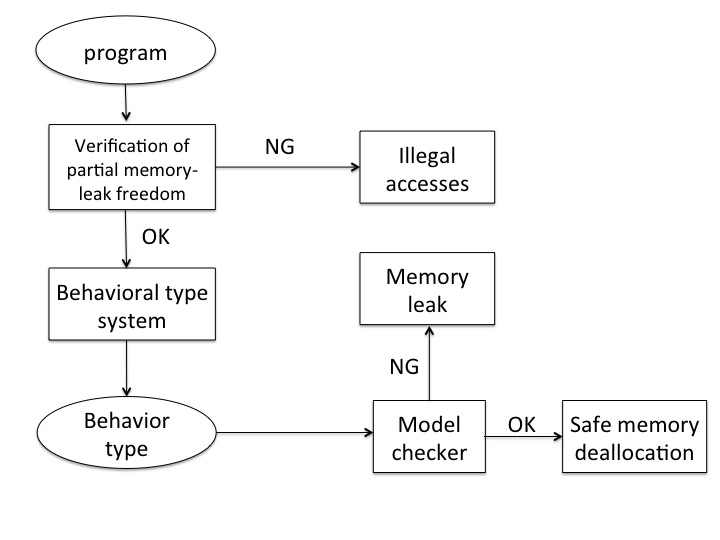
\includegraphics[width=10cm]{overview.jpg}
%% \caption{Overview of the algorithm}
%% \label{fig:ov}
%% \end{figure}

%% %% <<<<<<< HEAD
%% %% A program is first checked by $\mathbf{SK}$ type system; it is passed
%% %% to the behavioral type system proposed in our paper if its partial
%% %% correctness is guaranteed, otherwise returns ``it is not safe''; the
%% %% behavioral type system will check it and produce a behavioral type $P$
%% %% which abstracts the behavior of the program; and then by modeling the
%% %% behavioral type $P$ using model checkers like \texttt{SPIN} or
%% %% \texttt{CPAChecker} to verify whether the behavioral correctness of
%% %% the program is guaranteed. If its behavioral correctness is verified
%% %% by model checker, the safe memory deallocation for this program is
%% %% ensured, otherwise return ``it is not safe''.
%% %% =======
%% As represented in Figure~\ref{fig:ov}, a program is first checked by \textbf{SK} type system; if the properties about no double frees or illegal read/write operations to a deallocated memory cell is guaranteed, then it returns ``OK'' and the program is passed to our behavior type system, and it returns ``NG'' otherwise; our behavior type system will produce a behavioral type, and this behavioral type is passed to a model checker like \texttt{SPIN} or \texttt{CPAChecker} to verify whether it is consumed upper bound of memory cells.

%% Hence, by using our type system with \textbf{SK} type system, we can verify memory-leak freedom even for nonterminating programs.
%% %% >>>>>>> 9a92815042ab957eb9b2d406af7a45d4abb729b3

\paragraph{Notation} We write \(\vec{X}\) for a finite sequence of
\(X\).  We write \([\vec{x'}/\vec{x}]s\) for the term obtained by
replacing every free occurrences of \(\vec{x}\) in \(s\) with
\(\vec{x'}\).  We write \(\DOM(f)\) for the domain of the map \(f\).  For a
map \(f\), we write \(f \set{x \mapsto v}\) and \(f \bs x\) for the
maps defined as follows:
\[
\begin{array}{rcl}
f \set{x \mapsto v} (w) &=&
\left\{
\begin{array}{ll}
v & \mbox{if \(x = w\)}\\
f(w) & \mbox{otherwise.}
\end{array}
\right.\\
(f \bs x)(w) &=&
\left\{
\begin{array}{ll}
\mbox{undefined} & \mbox{if \(w \in \DOM(f)\)}\\
f(w) & \mbox{otherwise.}
\end{array}
\right.
\end{array}
\]


\section{Language \(\mathcal{L}\)}\label{sec:language}

This section gives the definition of language \(\mathcal{L}\), an
imperative language with memory allocation/deallocation primitives.
The language is essentially the same as one used by Sueanga et
al.~\cite{DBLP:conf/aplas/SuenagaK09}, where they propose a
type-based analysis for partial memory-leak freedom analysis.

The syntax of language \(\mathcal{L}\) is as follows.
\begin{eqnarray*}
  x,y,z,\dots \mbox{ (variables)} &\in& \VAR\\
  s \mbox{ (statements)} & ::= &  \SKIP \mid s_{1};s_{2} \mid *x \leftarrow y \mid \Free(x) \\
  & \mid & \LET x = \MALLOC \IN s \mid \LET x = \NULL\ \IN s  \\
  & \mid & \LET x = y \; \IN s \mid   \LET x = *y \; \IN s \\
  & \mid & \IFNULL(x) \; \THEN s_{1}\; \ELSE s_{2} \mid f(\vec{x})\\
  d \mbox{ (proc. defs.)} & ::= & \set{f \mapsto (x_1,\dots,x_n)s}\\
  D \mbox{(definitions) } &::=& \langle d_1 \cup \dots \cup d_n \rangle\\
  P \mbox{ (programs)} &::=& \langle D, s \rangle\\
\end{eqnarray*}

The language is equipped with procedure calls, dynamic memory
allocation and deallocation, and memory accesses with pointers.
\(\VAR\) is a countably infinite set of \emph{variables}.  The
statement \(\SKIP\) does nothing.  The statement \(s_1;s_2\) executes
\(s_1\) and \(s_2\) sequentially.  The statement \(*x \leftarrow y\)
writes \(y\) to the memory cell that \(x\) points to.  The statement
\(\LET x = e\ \IN s\) evaluates the expression \(e\), binds \(x\) to
the result, and executes \(s\).  The expression \(\Malloc()\)
allocates a new memory cell and evaluates to the pointer to the cell.
The expression \(\NULL\) evaluates to the null pointer.  The
expression \(y\) evaluates to its value.  The expression \(*y\)
evaluates to the value in the memory cell that \(y\) points to.  The
statement \(\IFNULL(x)\ \THEN\ s_1\ \ELSE\ s_2\) executes \(s_1\) if
\(x\) is \(\NULL\) and executes \(s_2\) otherwise.  The statement
\(f(\vec{x})\) calls procedure \(f\) with arguments \(\vec{x}\).

A procedure definition ranged over by \(d\) is a map from a procedure
name to an abstraction of the form \((\vec{x})s\).  We use a
metavariable \(D\) for a set of function definitions \(d_1 \cup \dots
\cup d_n\).  We assume that there are no duplicated definitions of
each function.  We also assume that there is no arity mismatch between
function definitions and function calls.  A program is a pair of
function definitions \(D\) and a main statement \(s\).


%% A program is a pair $(D,s)$, where $D$ is the set of definition.\\ The
%% command $\SKIP$ does nothing. The command $s_{1};s_{2}$ is executed as
%% a sequence, first executing $s_{1}$ and then $s_{2}$. The command $*x
%% \leftarrow y$ updates the content of the memory cell which is pointed
%% by pointer $x$ with value $y$. The command $\Free \Cirx$ deallocates
%% the memory cell which is pointed by a pointer $x$. Then command $\LET
%% x = e \; \IN s$ first evaluates the expression $e$ and binds the
%% return value of $e$ to $x$ and then executes statement $s$. The
%% command $\LET x = \Malloc \; \IN s$ first allocates a memory cell to a
%% pointer $x$ and then executes the statement $s$. The command $\LET x =
%% \NULL \IN s$ first allocates a null pointer to $x$ and then executes
%% $s$. The command $\LET x = y \; \IN s$ assign the pointer $y$ to $x$,
%% so the pointer $x$ and $y$ are said aliases for the same memory cell,
%% and then executes statement $s$. The command $\LET x = *y \; \IN s$
%% transfers a part of memory cells pointed by $y$ and then executes
%% statement $s$. The command $\IFNULL(x) \; \THEN s_{1} \; \ELSE s_{2}$
%% denotes that executing statement $s_{1}$ if pointer $x$ is a null
%% pointer, otherwise executing statement $s_{2}$. The command
%% $f(\vec{x})$ is a function call in which $\vec{x}$ denotes mutually
%% distinct variables like \{$x_{1}, \dots, x_{n}$\}. The notation $d$
%% denotes the definition of function $f(\vec{x})$ which has a body of
%% statement $s$. And examples are described by this syntax you can see
%% in Figure 1 and Figure 2.

\subsection{Operational semantics}
\label{sec:languageSemantics}

This section introduces the operational semantics of \(\mathcal{L}\).
We assume a countably infinite set \(\mathcal{H}\) of \emph{locations}
ranged over by \(l\).

We express a state of computation by \emph{configuration} \(\langle H,
R, s, n \rangle\).  A configuration consists of the following four
components:
\begin{itemize}
\item \(H\), a \emph{heap}, is a finite mapping from \(\mathcal{H}\)
  to \(\mathcal{H} \cup \set{\NULL}\);
\item \(R\), an \emph{environment}, is a finite mapping from \(\VAR\)
  to \(\mathcal{H} \cup \set{\NULL}\);
\item \(s\) is the statement that is being executed; and
\item \(n\) is a natural number that represents the number of memory
  cells available for allocation.
\end{itemize}
We later use \(n\) to formalize memory leaks caused by nonterminating
program.

The operational semantics is given by relation \(\langle H, R, s, n
\rangle \xlongrightarrow{\rho}_D \langle H', R', s', n' \rangle\)
where \(\rho\), an \emph{action}, is \(\Malloc\), \(\Free\), or
\(\tau\).  The action \(\Malloc\) expresses an allocation of a memory
cell; \(\Free\) expresses a deallocation; \(\tau\) expresses the other
actions.  We often omit \(\tau\) in \(\xlongrightarrow{\tau}_D\).  We
use a metavariable \(\sigma\) for a finite sequence of actions
\(\rho_1\dots\rho_n\).  We write
\(\xlongrightarrow{\rho_1\dots\rho_n}_D\) for
\(\xlongrightarrow{\rho_1}_D\xlongrightarrow{\rho_2}_D\dots\xlongrightarrow{\rho_n}_D\).
We write \(\xLongrightarrow{\rho}_D\) for
\(\xlongrightarrow{}_D^*\xlongrightarrow{\rho}_D\xlongrightarrow{}_D^*\).
We write \(\xLongrightarrow{\rho_1\dots\rho_n}_D\) for
\(\xLongrightarrow{\rho_1}_D\dots\xLongrightarrow{\rho_n}_D\).

%% Because we want to estimate the number of available memory cells at
%% every operation step, we extend the triple $\langle H\coma R\coma s
%% \rangle$ that is represented as run-time state in previous type system
%% to a quadruple $\langle H\coma R\coma s\coma n \rangle$ in our
%% paper. The introduced notation $n$ denotes the number of available
%% memory cells, a nature number. When executing the operation $\Malloc$,
%% the number of available memory cells will decrease 1, which is denoted
%% as ($n - 1$); when executing the operation $\Free$, the number of
%% available memory cells will increase 1, which is denoted as ($n +
%% 1$). The notation $H$, which models heap memory, is a mapping from
%% finite subset of $\mathcal{H}$ to $\mathcal{H}$ $\cup$ \{$null$\},
%% where $\mathcal{H}$ represents the set of \emph{heap addresses}. $R$,
%% which models registers, is a mapping from finite set of variables to
%% $\mathcal{H}$ $\cup$ \{$null$\}.

Figure~\ref{fig:transitionRules} defines the relation
%<<<<<<< HEAD
%% <<<<<<< HEAD
%% \(\xlongrightarrow{\rho}_D\). In the rule for \(\Free\), the \(\Free\) command correctly disposes  a memory cell which is pointed to by a pointer \(x\), and after doing \(\Free\) action, the number of available memory cells increases one.  In the rule for \(\Malloc\), the \(\Malloc()\) command need at least one cell for it to allocate a new memory cell \(l\) which is pointed to by the pointer \(x\), and after performing the \(\Malloc\) action, the number of available memory cells will decrease one.  The \(\bf MemEx\) for accessing null pointers or illegal accessing to a deallocated memory cell, and \(\OVERFLOW\) for performing allocation after running out of memory cells.
%
%% we require
%% that a memory cell has been allocated before deallocating it, and
%% after deallocating the memory cell from the heap \(H\), the number
%% \(n\) of available memory cells should increase one.  In the rule for
%% \(\Malloc\), the number of available memory cells should be positive;
%% the \(\Malloc\) command allocate e cell for allocates a new memory
%% cell \(l\) of which contents \(v\) can be any value in \(\mathcal{H}
%% \cup \set{\NULL}\) and reduces the number of available memory cells by
%% one. The \(\bf NullEx\) for accessing null pointers or illegal accessing to a
%% deallocated memory cell, and \(\OVERFLOW\) for performing allocation
%% after running out of memory cells.
%=======
\(\xlongrightarrow{\rho}_D\).  We add explanation to several important
rules.
\begin{itemize}
\item \rn{Sem-Free}: Deallocation of a memory cell pointed to by \(x\)
  is expressed by deleting the entry for \(R(x)\) from the heap.  This
  action increments the number of available cells (i.e., \(n\)) by one
  (i.e., \(n+1\)).
\item \rn{Sem-Malloc} and \rn{Sem-OutOfMem}: Allocation of a memory
  cell is expressed by adding a fresh entry to the heap.  This action is
  allowed only if the number of available cells is positive; if the
  number is zero, then the configuration leads to an error state
  \(\OVERFLOW\).
\item \rn{Sem-*Exn}: These rules express an illegal access to memory.
  If such action is performed, then the configuration leads to
  exceptional state \(\MEMEX\).  This state \(\MEMEX\) is not seen as
  an erroneous state in the current paper, hence is not excluded by
  the type system in Section~\ref{sec:typesystem}.
\end{itemize}


%>>>>>>> 5ea5427003cd6520f97c31833e1440ce3dff0481

\begin{figure}[p]
\begin{minipage}{\textwidth}

%% =======
%% %% Transition rules are listed in Figure 3. In these rules, $f\{x\to v\}$ is defined as a function $f'$ such that $f'(y) = v$ if $x = y$, otherwise $f'(y) = f(y)$ and $y \in dom(f)$. There are three rules about $\mathbf{NullEx}$ which denotes accessing a null pointer, three rules about $\mathbf{Error}$ for accessing a deallocated memory cell, and one rule about $\mathbf{Error}$ which denotes allocating a memory cell when there is no memory space.
%% %\begin{figure}[h]
%% % Skip Command
%% Runtime state is represented by $\langle H, R, s, n \rangle$, where $H$ is a mapping from finite subset of $\mathcal{H}$ to $\mathcal{H}$ $\cup$ \{$null$\}, in which $\mathcal{H}$ represents the set of \emph{heap addresses}, intuitively, the $H$ models a heap memory; $R$, which models registers, is a mapping from finite set of variables to $\mathcal{H}$ $\cup$ \{$null$\}.

%% Operational semantics are defined by the relations: $\rightarrow_{D}, \xlongrightarrow{\Malloc}_{D}, and \xlongrightarrow{\Free}_{D} $, in which $\xlongrightarrow{\Malloc}_{D}, and \xlongrightarrow{\Free}_{D} $ denote performing a allocation and deallocation operation respectively, and $\rightarrow_{D}$ expresses that performing an internal action like $\SKIP$ or assignment.
%% >>>>>>> 9a92815042ab957eb9b2d406af7a45d4abb729b3

\begin{minipage}{0.5\textwidth}
\infax[Sem-Skip]
{\langle H, R, \SKIP;s, n \rangle
\longrightarrow_{D}
\langle H, R, s, n \rangle}
\end{minipage}
\begin{minipage}{0.5\textwidth}
\infrule[Sem-Seq]
{\langle H, R, s_1, n \rangle \xlongrightarrow{\rho}_{D} \langle H', R', s_1', n' \rangle}
{\langle H, R, s_1;s_2, n \rangle \xlongrightarrow{\rho}_{D} \langle H', R', s_1';s_2, n' \rangle}
\end{minipage}

\infrule[Sem-LetNull]
{x' \notin \DOM(R)}
{\langle H\coma R\coma  \LET x = \NULL \ \IN s , n \rangle
  \longrightarrow_{D}
  \langle H\coma R\Lfc x' \mapsto \NULL \Rfc \coma   \Lb x'/x \Rb s , n  \rangle }

\infrule[Sem-LetEq]
{x' \notin \DOM(R)}
{\langle H\coma R\coma \LET x = y \; \IN s , n \rangle
  \longrightarrow_{D}
  \langle H\coma R\Lfc x' \mapsto R(y) \Rfc \coma   \Lb x'/x \Rb s , n  \rangle }

\infrule[Sem-IfNullT]
{R(x) = \NULL}
{\langle H \coma R \coma \IFNULL\Cirx\ \THEN   s_{1}\ \ELSE\  s_{2} \coma  n \rangle
  \longrightarrow_{D}
  \langle H\coma R\coma s_{1} \coma n \rangle}

\infrule[Sem-IfNullF]
{R(x) \neq \NULL}
{\langle H \coma R \coma \IFNULL\Cirx\ \THEN  s_{1}\ \ELSE  s_{2} \coma  n \rangle
  \longrightarrow_{D}
  \langle H\coma R\coma s_{2} \coma  n \rangle}

\infrule[Sem-Call]
{D(f) = (\vec{y})s}
{ \langle H\coma R\coma  f(\vec{x}) , n \rangle
  \longrightarrow_{D}
  \langle H\coma R\coma  \Lb \vec{x}/\vec{y} \Rb s , n \rangle}

\infax[Sem-Assign]
{ \langle H \set{R(x) \mapsto v}, R, *x \leftarrow y , n \rangle \xlongrightarrow{}_{D}
  \langle H \Lfc R(x) \mapsto R(y) \Rfc , R, \SKIP , n \rangle }

\infrule[Sem-LetDeref]
{x' \notin \DOM(R) \andalso R(y) \in \DOM(H)}
{\langle H\coma R\coma  \LET x = *y \; \IN s , n \rangle
  \longrightarrow_{D}
  \langle H\coma R\Lfc x' \mapsto H(R(y)) \Rfc \coma   \Lb x'/x \Rb s , n  \rangle }

\infax[Sem-Free] 
{\langle H\set{R(x) \mapsto v}\coma R\coma \Free(x) , n \rangle \xlongrightarrow{\Free}_{D}
  \langle H\backslash R(x) \coma R \coma \SKIP , n+1 \rangle}

\infrule[Sem-Malloc]
{l \notin \DOM(H) \andalso n > 0}
{\langle H\coma R\coma  \LET x = \Malloc() \; \IN s , n \rangle
  \xlongrightarrow{\Malloc}_{D}
  \langle H \Lfc l \mapsto v\Rfc \coma R\Lfc x' \mapsto l \Rfc \coma   \Lb x'/x \Rb s , n-1  \rangle }


\begin{minipage}{0.5\textwidth}
\infrule[Sem-AssignExn]
{R(x) = \NULL \mbox{ or } R(x) \notin \DOM(H)}
{\langle H\coma R\coma  *x \leftarrow y , n \rangle
  \longrightarrow_{D} \MEMEX }
\end{minipage}
\begin{minipage}{0.5\textwidth}
\infrule[Sem-DerefExn]
{R(y) = \NULL \mbox{ or } R(y) \notin \DOM(H)}
{\langle H\coma R\coma  \LET x = *y \; \IN s, n \rangle
    \longrightarrow_{D} \MEMEX}
\end{minipage}

\infrule[Sem-FreeExn]
{R(x) = \NULL \mbox{ or } R(x) \notin \DOM(H)}
{\langle H\coma R\coma \Free(x) , n \rangle \xlongrightarrow{\Free}_{D} \MEMEX}

\infax[Sem-OutOfMem]
{ \langle H\coma R\coma \LET x = \Malloc() \ \IN s ,  0  \rangle    \xlongrightarrow{\Malloc}_{D}
     \OVERFLOW}

\end{minipage}

\caption{Operational semantics of \(\mathcal{L}\).}
\label{fig:transitionRules}
\end{figure}

%% Transition rules are listed in Figure 3. In these rules, $f\{x\to v\}$
%% is defined as a function $f'$ such that $f'(y) = v$ if $x = y$,
%% otherwise $f'(y) = f(y)$ and $y \in dom(f)$. There are three rules
%% about $\mathbf{NullEx}$ which denotes accessing a null pointer, three
%% rules about $\mathbf{Error}$ for accessing a deallocated memory cell,
%% and one rule about $\mathbf{Error}$ which denotes allocating a memory
%% cell when there is no memory space.
%% %\begin{figure}[h]
%% % Skip Command
%% Runtime state is represented by $\langle H, R, s, n \rangle$, where
%% Operational semantics is defined by the relations\\
%% $\rightarrow_{D}, \xlongrightarrow{\Malloc}_{D}, and \xlongrightarrow{\Free}_{D} $ defined by the rules in ....\\
%% Here, $\rightarrow_{D}$ expresses; ....\\

%% $$
%%     \frac{n \in \mathbb{N}}
%%             {\langle H\coma R\coma  \SKIP;s , n \rangle
%%               \longrightarrow_{D}
%%                 \langle H\coma R\coma   s , n \rangle }
%%      \Rtab \mbox{(E-Skip)}
%% $$
%% % Assignment
%% $$
%%      \frac{R(x) \in dom(H), n \in \mathbb{N}}
%%            {\langle H\coma R\coma  *x \leftarrow y , n \rangle
%%              \longrightarrow_{D}
%%              \langle H \Lfc R(x) \rightarrow R(y) \Rfc \coma R \coma   \SKIP , n  \rangle }
%%      \Rtab \mbox{(E-Assign)}
%% $$
%% % Free Command
%% $$
%%      \frac{R(x) \in dom(H) , n \in \mathbb{N}}
%%           {\langle H\coma R\coma  \FREE , n \rangle
%%             \xlongrightarrow{\Free}_{D}
%%             \langle H\backslash \Lfc R(x) \Rfc \coma R \coma   \SKIP , n+1  \rangle }
%%      \Rtab \mbox{(E-Free)}
%% $$
%% % Let Null Command
%% $$
%%      \frac{x' \notin dom(R)}
%%            {\langle H\coma R\coma  \LET x = \NULL \IN s , n \rangle
%%              \longrightarrow_{D}
%%              \langle H\coma R\Lfc x' \rightarrow \NULL \Rfc \coma   \Lb x'/x \Rb s , n  \rangle }
%%      \Rtab \mbox{(E-LetNull)}
%% $$
%% % Let Eq Command
%% $$
%%      \frac{x' \notin dom(R)}
%%             {\langle H\coma R\coma \LET x = y \; \IN s , n \rangle
%%               \longrightarrow_{D}
%%               \langle H\coma R\Lfc x' \rightarrow R(y) \Rfc \coma   \Lb x'/x \Rb s , n  \rangle }
%% \Rtab \mbox{(E-LetEq)}
%% $$
%% % Reference Command
%% $$
%%      \frac{x' \notin dom(R)}
%%             {\langle H\coma R\coma  \LET x = *y \; \IN s , n \rangle
%%               \longrightarrow_{D}
%%               \langle H\coma R\Lfc x' \rightarrow H(R(y)) \Rfc \coma   \Lb x'/x \Rb s , n  \rangle }
%%      \Rtab \mbox{(E-LetDref)}
%% $$
%% % Malloc (allocate) Command
%% $$
%%      \frac{h \notin dom(H)}
%%             {\langle H\coma R\coma  \LET x = \Malloc() \; \IN s , n \rangle
%%               \xlongrightarrow{\Malloc}_{D}
%%               \langle H \Lfc h \rightarrow v\Rfc \coma R\Lfc x' \rightarrow h \Rfc \coma   \Lb x'/x \Rb s , n-1  \rangle }
%% \Rtab \mbox{(E-Malloc)}
%% $$
%% % IFNULL T
%% $$
%%     \frac{R(x) = \NULL}
%%            {\langle H \coma R \coma \IFNULL\Cirx   \THEN   s_{1} \ELSE\  s_{2} \coma  n \rangle
%%            \longrightarrow_{D}
%%            \langle H\coma R\coma s_{1} \coma n \rangle}
%%     \Rtab \mbox{(E-IfNullT)}
%% $$
%% % IFNULL F
%% $$
%%     \frac{R(x) \neq \NULL}
%%            {\langle H \coma R \coma \IFNULL\Cirx \THEN  s_{1} \ELSE  s_{2} \coma  n \rangle
%%            \longrightarrow_{D}
%%            \langle H\coma R\coma s_{2} \coma  n, \rangle}
%%     \Rtab \mbox{(E-IfNullF)}
%% $$
%% % Function Call
%% $$
%%      \frac{f(\vec{y}) = s \in D}
%%             { \langle H\coma R\coma  f(\vec{x}) , n \rangle
%%                \longrightarrow_{D}
%%                \langle H\coma R\coma  \Lb \vec{x}/\vec{y} \Rb s , n \rangle}
%%       \Rtab \mbox{(E-Call)}
%% $$
%% % Error : access the null memory cell
%% $$
%%       \frac{R(x) = null}
%%             {\langle H\coma R\coma  *x \leftarrow y , n \rangle
%%               \longrightarrow_{D}
%%              \bf NullEx }
%%       \Rtab \mbox{(E-AssignNullError)}
%% $$
%% % ERROR : access the null memory cell
%% $$
%%       \frac{R(y) = null}
%%              {\langle H\coma R\coma  x = *y, n \rangle
%%                \longrightarrow_{D}
%%               \bf NullEx }
%%              \Rtab \mbox{(E-DrefNullError)}
%% $$
%% $$
%%      \frac{R(x) =  null }
%%            {\langle H\coma R\coma  \FREE , n \rangle
%%              \xlongrightarrow{\Free}_{D} \bf NullEx  }
%%       \Rtab \mbox{(E-FreeNullError)}
%% $$
%% % ERROR :
%% $$
%%      \frac{R(x) \notin dom(H) \cup \Lfc null \Rfc}
%%            {\langle H\coma R\coma   *x \leftarrow y,  n \rangle
%%              \longrightarrow_{D}
%%            \bf  Error }
%%     \Rtab \mbox{(E-AssignError)}
%% $$
%% % ERROR
%% $$
%%       \frac{R(y) \notin dom(H) \cup \Lfc null \Rfc}
%%            {\langle H\coma R\coma  \LET x  = *y \; \IN s, n \rangle
%%               \longrightarrow_{D}
%%                 \bf  Error }
%%       \Rtab \mbox{(E-DrefError)}
%% $$
%% %
%% $$
%%       \frac{R(x) \notin dom(H) \cup \Lfc null \Rfc}
%%             {\langle H\coma R\coma  \FREE , n \rangle
%%               \xlongrightarrow{\Free}_{D}
%%               \bf Error }
%%      \Rtab \mbox{(E-FreeError)}
%% $$
%%  % ERROR: no enough space
%% $$
%%       \langle H\coma R\coma \LET x = \Malloc() \ \IN s ,  0  \rangle
%%       \xlongrightarrow{\Malloc}_{D}
%%       \mathbf{Error}
%%       \Rtab \mbox{(E-MallocError)}
%% $$
%% $$
%%      \mathbf{Figure \; 3.} \;\;  \mbox{ Operational Semantics}
%% $$
%
%\caption{Operational Semantics.}
%\label{example:os}
     %\end{figure}

As mentioned in Section~\ref{sec:introduction}, a program is said to
leak memory if it consumes unbounded number of memory cells.
Formally, this is defined as follows.

\begin{myDef}[Memory leaks]
\label{df:ml}
%% memory leaks:\\
%% if $\vdash \langle D, s \rangle : n$, then $\langle \emptyset, \emptyset, s, n \rangle \xlongrightarrow{\rho_{1}, \dots, \rho_{n}}_{D} \langle H, R, s', 0 \rangle \xlongrightarrow{\Malloc}_{D} Overflow $\\
%% memory-leak \ freedom: $\exists n \in \mathbb{N}$ s.t. $\langle \emptyset, \emptyset, s, n \rangle \nrightarrow^{*}Overflow$
A configuration \(\langle H, R, s, n \rangle\) \emph{goes overflow} if
there is \(\sigma\) such that \(\langle H, R, s, n \rangle
\xLongrightarrow{\sigma} \OVERFLOW\).  A program \(\langle D, s
\rangle\) \emph{requires at least \(n\) cells} if \(\langle \emptyset,
\emptyset, s, n \rangle\) goes overflow.  A program \(\langle D, s
\rangle\) is \emph{totally memory-leak free} if there is a natural
number \(n\) such that it does not require more than \(n\) cells.
\end{myDef}


\section{Type system}
\label{sec:typesystem}

\subsection{Types}

The syntax of the types is as follows.
\[
\begin{array}{rlcl}
  P & (\mbox{behavioral types})&::=& {\bf 0} \tB P_{1};P_{2} \tB P_{1}+P_{2} \tB \Malloc \tB \Free \tB \alpha \tB \mu\alpha.P \\
  \Gamma & (\mbox{variable type environments}) &::=& \set{x_1, x_2, \dots, x_n}\\
  \Theta & (\mbox{function type environments}) &::=& \set{f_1\COL P_1,\dots,f_n\COL P_n}\\
\end{array}
\]
We use metavariable \(P\) for \emph{behavioral types}, which are
abstractions of the behavior of programs.  The type ${\bf 0}$
%<<<<<<< HEAD
%% represents the do-nothing behavior.  The type \(P_1;P_2\) represents
%% the sequential execution of \(P_1\) and \(P_2\).  The type \(P_1 +
%% P_2\) represents the choice between \(P_1\) and \(P_2\).  The type
%% \(\Malloc\) represents an allocation a memory cell exactly once.  The
%% =======
represents do-nothing behavior.  The type \(P_1;P_2\) represents the
sequential execution of \(P_1\) and \(P_2\).  The type \(P_1 + P_2\)
represents the choice between \(P_1\) and \(P_2\).  The type
\(\Malloc\) represents an allocation of a memory cell exactly once.  The
%>>>>>>> 4423a1ce9aed6c247aa532bd4d789da44f8e4939
type \(\Free\) represents a deallocation.  \(\alpha\) is a type
variable. The type \(\mu \alpha.P\) represents the behavior of
\(\alpha\) defined by the recursive equation \(\alpha = P\).

Type environments for variables, ranged over by \(\Gamma\), are set of
variables.  Since our interest is the behavior of a program, not the
types of values, a variable type environment does not carry
information on the types of variables.  We also designate type
environments for function names ranged over by \(\Theta\).  A function
type environment carries information on the behavior of functions
represented by behavioral types.  We often omit the curly braces
around variable and function environments.

%% For example, given \(\Malloc;\alpha;\Free\) as \(P\), a recursive type
%% is of the form \(\mu \alpha. \Malloc;\alpha;\Free\) and can go further
%% as \(\Malloc;(\mu\alpha.\Malloc;\alpha;\Free);\Free\).

%%  $P_{1};P_{2}$ is for sequential execution. $P_{1} + P_{2}$
%% is abstracted as conditional. $\Malloc$ is the behavior of a statement
%% that allocates a memory cell exactly once. $\Free$ is for deallocating
%% memory cell exactly once. $\mu \alpha. P$ is a recursive type. For
%% example, the behavior of the body of function $h$ in Figure~\ref{ex:np} is
%% abstracted as $\mu
%% \alpha. \Malloc;\Malloc;\Free;\Free;\alpha$. $\alpha$ is a type
%% variable and bounded to the recursive constructor $\mu \alpha$.

%% The function type is described as $(\tau_{1}, \dots, \tau_{n})P$,
%% which means a function receives some pointers as arguments and its
%% body is abstracted as a behavioral type $P$.

% Semantics of Behavioral Types %
% \subsection{Semantics of behavioral types}


\begin{figure}[t]

\begin{minipage}[t]{0.25\textwidth}
\infax[Tr-Skip]
{\mathbf{0};P \xlongrightarrow{\tau} P}
\end{minipage}
\begin{minipage}[t]{0.34\textwidth}
\infax[Tr-Malloc]
{\Malloc \xlongrightarrow{\Malloc} {\bf 0}}
\end{minipage}
\begin{minipage}[t]{0.3\textwidth}
\infax[Tr-Free]
{\Free \xlongrightarrow{\Free} {\bf 0}}
\end{minipage}

\vspace{2mm}

\begin{minipage}{0.33\textwidth}
\infax[Tr-Rec]
{\mu \alpha.P \xlongrightarrow{\tau}  [\mu \alpha . P/\alpha]  P}
\end{minipage}
\begin{minipage}{0.3\textwidth}
\infax[Tr-ChoiceL]
{P_{1} + P_{2} \xlongrightarrow{\tau} P_{1}}
\end{minipage}
\begin{minipage}{0.33\textwidth}
\infax[Tr-ChoiceR]
{P_{1} + P_{2} \xlongrightarrow{\tau} P_{2}}
\end{minipage}

\infrule[Tr-Seq]
{P_{1} \xlongrightarrow{\rho} P_{1}' }
{P_{1};P_{2} \xlongrightarrow{\rho} P_{1}';P_{2}}
\caption{Semantics of behavioral types.}
\label{fig:semBTypes}
\end{figure}

%% The notation $\rightarrow$ denotes that a behavioral type can be
%% reduced by the internal action. Notation $\xlongrightarrow{\alpha}$
%% means that a behavioral type can be reduced by executing $\alpha$
%% actions, and the $\alpha$ here is $\{\Malloc, \Free\}$.

The semantics of behavioral type are given by the labeled transition
system in Figure~\ref{fig:semBTypes}.  \(P \xlongrightarrow{\rho} P'\)
means that \(P\) can make an action \(\rho\) and, after \(P\) make the
action \(\rho\), \(P\) turns into \(P'\).

%% The behavioral types \(\Malloc\) and \(\Free\), intuitively, just
%% perform \(\Malloc\) and \(\Free\) actions respectively.  For the
%% type \(P_1 + P_2\), it only makes a choice between \(P_1\) and
%% \(P_2\), so it performs the internal action and then behave like
%% either \(P_1\) or \(P_2\).  The type \(\mu \alpha.P\) performs
%% nothing but substitution, so it makes an internal action and
%% behaves like a substitution \([\mu\alpha.P/\alpha]P\). For the
%% behavioral type \(P_1;P_2\), \(P_1\) make actions \(\rho\) until it
%% turns into \(0\); The type \(\bf{0};P_2\) The type \(\bf 0\)
%% represents do-nothing behavior, so the type \(\bf{0}\)\(;P\) should
%% perform an internal action \(\tau\) and then behave like the
%% following behavior \(P\). For the type \(\Malloc\) and \(\Free\),
%% they should perform \(\Malloc\) and \(\Free\) actions respectively
%% and, after performing actions they do nothing, so the following
%% behaves like \(\bf 0\). For the type \(P_1 + P_2\), it only makes a
%% choice between \(P_1\) and \(P_2\) and do nothing else, so it
%% performs the internal action and then behave like either \(P_1\) or
%% \(P_2\). The type \(\mu \alpha.P\) performs nothing but
%% substitution, so it makes an internal action and behaves like a
%% substitution \([\mu\alpha.P/\alpha]P\).

% Type Judgments

\subsection{Typing rules}

%%  We design the type system so that
%% this type judgment implies the property: when $s$ executes
%% $\Malloc$(resp.$\Free$), then $P$ is equivalent to
%% $\Malloc;P'$(resp.$\Free;P'$) for a type $P'$ such that $\Theta;
%% \Gamma \vdash s': P'$, where $s'$ is the continuation of $s$. This
%% property guarantees the behavioral type soundly abstracts the upper
%% bound of the consumed memory cells.

%% Typing rules are presented in Figure~\ref{fig:typingrules}. In the rule for assignment, the behavior of  $*x \leftarrow y$ is $\bf 0$. The rule for $\Free$ represents that the behavior of $\Free \Cirx$ is $\Free$. The rule T-Malloc represents that $\LET x = \MALLOC \; \IN s$ has the behavior $\Malloc;P$, where $P$ is the behavior of statement $s$. The rule for function call represents that function $f$ has the behavior $P$ which is the behavior of the body of this function .

%% \(\vdash D \COL \Theta\) denotes that the set \(D\) of definitions
%% has a type \(\Theta\).

We need several auxiliary definitions to present typing rules.  We
first define predicate \(\OK_n(P)\) that means that \(P\) describes
the behavior of a program that requires at most \(n\) memory cells.

\begin{myDef}[\(\sharp_{\rho}(\sigma)\)]
 \label{df:sharf}
\(\sharp_{\rho}(\sigma)\) is the number of \(\rho\) in the sequence
\(\sigma\).
\end{myDef}

%% begin{myDef}[OK(P)]
%%  \(OK_n(P)\) holds if a program executes sequence actions \( \sigma\) for any \(P'\) such that \(P\xLongrightarrow{\sigma}P'\), then the difference of \( \sharp_{malloc}(\sigma)\) and \( \sharp_{free}(\sigma)\) does not exceed the number \(n\).
%% \label{df:okn}
%% \
%%end{myDef}[OK_n(P)]

\begin{myDef}
\label{df:okn}
\(OK_{n}(P)\) holds if, for any \(P'\), if \(P
\xlongrightarrow{\sigma}P'\) then
\(\sharp_{malloc}(\sigma)-\sharp_{free}(\sigma)\le n\).
\end{myDef}

We also define subtyping.  Following the idea of Kobayashi et
al.~\cite{DBLP:journals/tcs/IgarashiK04}, we define subtyping by
using simulation between behavioral types.

 \begin{myDef}[Subtyping]
% $P_{1} \le P_{2}$ represents that $P_{1}$ is the subtype of $P_{2}$ and  means that:

\(P_1 \le P_2\) is the largest relation such that, for any \(P_1'\)
and \(\rho\), if \(P_1 \xlongrightarrow{\rho} P_1'\), then there
exists \(P_2'\) such that \(P_2 \xLongrightarrow{\rho} P_2'\) and
\(P_2 \le P_2'\).

\label{df:subtype}
\end{myDef}
%% At the end of $s$, memory leak freedom is guaranteed by $OK_{n}(P)$ ,where $P$ is the behavior of $s$. $OK_{n}(P)$ is defined as Definition~\ref{df:okn} in which $\sharp_{malloc}(\alpha)$ and $\sharp_{free}(\alpha)$ are functions to count the number of $\Malloc$ and $\Free$ actions in $\alpha$ respectively. This definition, intuitively, means at every running step the number of allocated memory cells will never go out of memory scope.
%% \begin{myDef}
%%   $OK_{n}(P) \iff \forall P',\; P \xlongrightarrow{\alpha}^{*}P'$ then $\sharp_{malloc}(\alpha)-\sharp_{free}(\alpha)\le n$.
%% \label{df:okn}
%% \end{myDef}

\begin{figure}[tp]
\begin{minipage}{\textwidth}

\begin{minipage}{0.5\textwidth}
\infax[T-Skip]
{\Theta ; \Gamma \vdash \SKIP : \mathbf{0}}
\end{minipage}
\begin{minipage}{0.5\textwidth}
\infrule[T-Seq]
{\Theta ; \Gamma \vdash s_{1} : P_{1} \Rtab \Theta ; \Gamma \vdash s_{2} : P_{2}}
{\Theta ; \Gamma \vdash s_{1} ; s_{2} : P_{1};P_{2} }
\end{minipage}

\vspace{2mm}

\begin{minipage}{0.5\textwidth}
\infax[T-Assign]
{\Theta ; \Gamma, x, y \vdash *x \leftarrow y : \mathbf{0} }
\end{minipage}
\begin{minipage}{0.5\textwidth}
\infax[T-Free]
{\Theta ; \Gamma, x \vdash \Free(x) : \Free}
\end{minipage}

\vspace{2mm}

\begin{minipage}{0.5\textwidth}
\infrule[T-Malloc]
{\Theta ; \Gamma,x \vdash s : P}
{\Theta ; \Gamma \vdash \LET x = \MALLOC \; \IN s  : \Malloc;P}
\end{minipage}
\begin{minipage}{0.5\textwidth}
\infrule[T-LetEq]
{\Theta ; \Gamma , x, y  \vdash s : P}
{\Theta ; \Gamma, y \vdash \LET x = y \; \IN s : P}
\end{minipage}

\vspace{2mm}

\begin{minipage}{0.5\textwidth}
\infrule[T-LetDeref]
{\Theta ; \Gamma , x, y  \vdash s : P}
{\Theta ; \Gamma, y \vdash \LET x = *y \; \IN s : P}
\end{minipage}
\begin{minipage}{0.5\textwidth}
\infrule[T-LetNull]
{\Theta ; \Gamma, x  \vdash s : P}
{\Theta ; \Gamma \vdash \LET x = \mathbf{null} \; \IN s : P}
\end{minipage}

\vspace{2mm}

\begin{minipage}{0.5\textwidth}
\infrule[T-IfNull]
{\Theta ; \Gamma, x \vdash s_{1} : P \andalso \Theta ; \Gamma, x \vdash s_{2} : P}
{\Theta ; \Gamma, x \vdash \IFNULL(x) \; \THEN s_{1}\; \ELSE s_{2} : P}
\end{minipage}
\begin{minipage}{0.5\textwidth}
\infax[T-Call]
{\Theta, f \COL P; \Gamma, \vec{x} \vdash f(\vec{x}) : P}
\end{minipage}

\vspace{2mm}

\infrule[T-Sub]
{\Theta ; \Gamma \vdash s : P_{1} \andalso P_{1} \le P_{2}}
{\Theta ; \Gamma \vdash s : P_{2}}

\infrule[T-Def]
{\DOM(D) = \DOM(\Theta)
\andalso
\Theta; x_1,\dots,x_n \vdash s \COL \Theta(f)
\mbox{ for each \(f \mapsto (x_1,\dots,x_n)s \in D\).}
}
{\vdash D \COL \Theta}
% Program
\infrule[T-Program]
{\vdash D : \Theta \andalso \Theta; \emptyset\vdash s : P \Rtab OK_{n}(P)}
{\vdash \langle D, s \rangle : n}

\end{minipage}
\caption{Typing rules.}
\label{fig:typingrules}
\end{figure}

The type judgment for statements is of the form $\Theta ; \Gamma
\vdash s : P$.  It expresses that, under the variable type environment
\(\Gamma\) and the function type environment \(\Theta\), the behavior
of $s$ is abstracted by behavior $P$.

%% \todo{Rewrite this paragraph} Figure~\ref{fig:typingrules} shows the
%% typing rules of our type system. In the rule for assignment, the
%% expression behaves like \(\bf 0\) . In the rule for \(\Free\), it
%% performs an allocation, so it behaves like \(\Free\).  In the rule for
%% \(\Malloc\), this let-expression performs an allocation and then
%% executes the statement \(s\), so its behavior like \(\Malloc;P\) where
%% the \(P\) is the behavior type of statement \(s\). In the rule for
%% other let-expressions like \rn{Tr-LetEq}, \rn{Tr-LetDref} and
%% \rn{Tr-LetNull}, they do not perform any allocation and deallocation,
%% so they behave like \(P\) which is the behavior of statement \(s\).

Figure~\ref{fig:typingrules} shows the typing rules.  It should be
easy to observe correspondence between a construct in a statement and
that in the behavioral type assigned to the statement.  For example,
rule \rn{T-Malloc} expresses that the behavior of \(\LET x =
\Malloc()\ \IN s\) is abstracted by \(\Malloc; P\) where \(P\) is the
behavior of \(s\); this statement first allocates a memory cell once,
and then executes \(s\).

\(\vdash D \COL \Theta\) is the judgment for function definitions.
This judgment represents that the behavior assigned to each function
symbol \(f\) in \(\Theta\) indeed abstracts the behavior of its
function body.  This property is guaranteed by \rn{T-Def}.

%<<<<<<< HEAD
%T%% ype judgment for programs, \(\vdash \langle D, s \rangle \COL n\),
%% expresses that the program requires at most \(n\) memory cells when it
%% is run.  In order to guarantee this, rule \rn{T-Prog} forces a side
%% condition \(\OK_n(P)\) where \(P\) is a behavioral type assigned to
%% \
%%(s\) under \(\Theta\) assigned to \(D\).
%=======
The type judgment for programs, \(\vdash \langle D, s \rangle \COL n\),
expresses that the program does not require more than \(n\) memory
cells when it is run.  In order to guarantee this, rule \rn{T-Prog}
forces a side condition \(\OK_n(P)\) where \(P\) is a behavioral type
assigned to \(s\) under \(\Theta\) assigned to \(D\).
%>>>>>>> 4423a1ce9aed6c247aa532bd4d789da44f8e4939

\subsection{Type soundness}

% This subsection describes some theorems and lemmas for type safety.

The following theorem states soundness of the type system.  The proof
is in the full version~\cite{fullversion}.

\begin{theorem}\label{thm1}
If $\vdash \langle D, s \rangle : n$ for some \(n\), then \(\langle D,
s \rangle\) is totally memory-leak free.
\end{theorem}

% This theorem says that a well typed program guarantees memory leak
% freedom.

The proof is based on the following lemmas: preservation and lack of
immediate overflow.

\begin{lemma}[Preservation]
\label{lem:preservation}
If $OK_{n}(P)$, $\Theta; \Gamma \vdash s : P$, \(\vdash D \COL
\Theta\), and $\langle H,R,s,n \rangle \xlongrightarrow{\rho} \langle
H',R',s', n' \rangle$, then there exists $P'$ such that (1) $ \Theta;
\Gamma \vdash s' : P'$, (2) \(P \xLongrightarrow{\rho} P'\), and (3)
\(OK_{n'}(P')\).
\end{lemma}

%% \begin{lemma}[Preservation $\mathbf{II}$]%\label{preser}
%% If $OK_{n}(P)$, $\Theta ; \Gamma \vdash s : P$ and $\langle H,R,s,n \rangle
%% \rightarrow \langle H',R',s', n'
%% \rangle$, then $\exists P'$ s.t. \\
%% (1) $\Theta; \Gamma \vdash s' : P'$\\
%% (2) $ P \rightarrow^{*} P'  $\\
%% (3) $OK_{n'}(P')$
%% \end{lemma}

\begin{lemma}[Lack of immediate overflow]
\label{lem:immediateSafety}
If $\Theta; \Gamma \vdash s \COL P$, \(\vdash D \COL \Theta\), and
\(\OK_n(P)\), then $\langle H, R, s, n \rangle
\not\xlongrightarrow{\Malloc} \OVERFLOW$.
\end{lemma}

\section{Type reconstruction}
\label{sec:reconstruction}

%% This section describes how to construct syntax directed typing rules
%% according to the typing rules of above section, and it provides an
%% algorithm which inputs statements and returns a pair containing
%% constraints and behavior types.

This section describes a type reconstruction procedure for the type
system in Section~\ref{sec:typesystem}.  Since the procedure is
essentially the same as one in Kobayashi et
al.~\cite{DBLP:journals/lmcs/KobayashiSW06}, we do not give a concrete
definition here.  The procedure described here is not complete.  We
could reject a program that is well-typed in the type system.

The reconstruction procedure is a constraint-based one.  It generates,
given a program, constraints for the program to be well-typed by
constructing a derivation tree based on the rules in
Figure~\ref{fig:typingrules}.  A constraint is either a subtyping
constraint \(\alpha \ge P\), or \(\OK_\nu(\alpha)\), where \(\nu\) is
a symbol for an unknown natural number.  Since \rn{T-Prog} is the only
place where the condition \(\OK_n(P)\) is involved, the constraint set
includes exactly one constraint of the form \(\OK_\nu(\alpha)\).  The
concrete definition of the constraint generation is in the full
version~\cite{fullversion}.

By using the result obtained by Kobayashi et al.~\cite[Lemma
  3.8]{DBLP:journals/lmcs/KobayashiSW06}, a subtyping constraint
\(\alpha \ge P\) can be resolved by setting \(\alpha = \mu
\alpha. P\), which is the least solution of the constraint.  Hence,
the generated constraint set is reduced to a single constraint
\(\OK_{\nu}(P')\) for some behavioral type \(P'\).

By definition, \(\OK_{\nu}(P)\) holds if there is a natural number
\(n\) such that, for all \(\sigma\) and \(P'\), \(P
\xlongrightarrow{\sigma} P'\) implies \(\sharp_{\Malloc}(\sigma) -
\sharp_{\Free}(\sigma) \le n\).  In order to check this condition
soundly, we fix the upper bound of \(\nu\) to be checked.  Then,
\(\OK_{\nu}(P)\) can be checked by model-checking a system with
finitely many states; hence, model checkers like
CPAChecker~\cite{beyer2011cpachecker} and
SPIN~\cite{holzmann2004spin,ben2008principles} are
applicable.  More detailed description on how we apply a
model-checking algorithm to check \(\OK_\nu(P)\) is in the forthcoming
version.

%% \subsection{Constraint generation}

%% %% By syntax directed typing rules, the type reconstruction algorithm has
%% %% been designed as in Figure~\ref{fig:tyin}.

%% %% Function $PT_{v}(x) = (C,\emptyset)$ denotes that it receives a
%% %% pointer variable $x$ and outputs a pair consisting of
%% %% constraints set $C$ and an empty set. $PT_{\Theta}(s) = (C, P)$
%% %% is a mapping from statements to a pair -- constraints set $C$
%% %% and behavioral types $P$, where $\Theta$ is mapping from
%% %% function names to function types. $PT(\langle D,s \rangle) = (C,
%% %% P)$ denotes that it receives a program and produces a pair $(C,
%% %% P)$. $\alpha_{i}$ and $\beta$ are fresh type variables.



%% \subsection{Constraints reduction} $PT\langle D, s \rangle$
%% receives a program as argument and produces a pair which consists
%% of the subtype constraints on behavior types of the form $\alpha
%% \ge A$, and constraints of the form $OK_{n}(P)$. Thus, we obtain
%% the following constraints:\\ $$ \{ \alpha_{1} \ge A_{1}, \dots,
%% \alpha_{n} \ge A_{n}, OK_{n}(P)\} $$ Here, we can assume that
%% $\alpha_{1}, \dots, \alpha_{n}$ are pairwise-distinct, since
%% $\alpha \ge A_{1}$ and $\alpha \ge A_{2}$ can be replaced with
%% $\alpha \ge A_{1}+A_{2}$ by lemma 3.8 in
%% paper~\cite{DBLP:journals/lmcs/KobayashiSW06}. we can also assume
%% that $\{ \alpha_{1}, \dots, \alpha_{n} \}$ contains all the type
%% variables in the constraints, since otherwise we can always add the
%% tautology $\alpha \ge \alpha$. Each subtype constraints $\alpha \ge
%% A$ can be replaced by $\alpha \ge \mu \alpha. A$, by lemma
%% 3.8(4)~\cite{DBLP:journals/lmcs/KobayashiSW06} ( substituting
%% $\alpha$ for $B$ in this lemma). Therefore the above constraints
%% can be further reduced to $OK_{n}([\vec{A} \slash
%% \vec{\alpha}]P)$. Here, $A'_{1}, \dots, A'_{n}$ are the least
%% solutions for the subtype constraints.

%% \section{Preliminary Experiment}

\section{Preliminary Experiments}
\label{sec:experiment}
In this section, we did the experiments by comparing applying a model
checker to original C language programs with to abstracted
behavior. Table~\ref{tb:mcc} and Table~\ref{tb:mca} show the results
of the experiments. All of the experiments are done on a machine with
an Intel(R) Core(TM) i7-3770 CPU @ 3.40GHz, 8MB cache and 3.76GB memory, running
on Debian (kernel version 2.6.32-5-amd64) and CPAchecker (version 1.3.4).

In these two tables, the meaning of each column is described as
follows. The column \texttt{original programs} and \texttt{abstracted
  behavior}, which mean applying the model checker to a original C
language program and to abstracted behavior respectively. These two
columns consist of several columns: $\sharp$\texttt{loc} means the
number of program locations; $\sharp$\texttt{fun} means the number of
functions in a program; \texttt{cpu time (total)} means the total
execution time of CPU in seconds; \texttt{memory(MB)} means the number
of virtual memory cells consumed by model checker in \texttt{MByte};
\texttt{fixed num} means the number of available memory cells which we
fix; the \texttt{TRUE} in the \texttt{verified result} column means
the number of the memory cells which a program consumes does not
exceed the \texttt{fixed num}, otherwise it is \texttt{FALSE} which
denoates memory-leak.

The programs used for the experiments are described as follows:[TODO]
\begin{itemize}
%% \item \texttt{linklist.c} and \texttt{linklist2.c} initialize a list,
%%   and perform some operations on the list (insert , delete, locate a
%%   node and traverses the list), and destroy the list. The difference
%%   between \texttt{linklist.c} and \texttt{linklist2.c} is that the
%%   former creates list by the head-insertion, whereas the latter creates a list
%%   by the tail-insertion.
%% \item \texttt{linkstack.c} creates a stack, pushes some elements in
%%   the stack, traverses the stack and clear the stack.
%% \item \texttt{linkqueue.c} initializes a queue, inserts, deletes some
%%   elements in the queue, clears the queue and destroys the queue.
%% \item \texttt{binarysorttree.c} inserts some nodes in a binary tree
%%   and deletes all the allocated nodes.
\item \texttt{database.c} models a database. It opens a database and
  performs some operations on the database (retrieve, delete and
  update data, or create a new database) and closes the database. We
  rewrite this program as \texttt{database\_rw.c}.
%% \item \texttt{ihex2fw.c} is a file from Linux kernel
%%   \texttt{/firmware/ihex2fw.c}, which converts ihex files into binary
%%   representation for use by Linux kernel.
%% \item \texttt{gen\_init\_cpio.c} is a file from Linux kernel
%%   \texttt{/usr/gen\_init\_cpio.c}, which produces a binary file which
%%   performs on a file containing newline separated entries that
%%   describe the files to be included in the initramfs archive.
\end{itemize}

The results present in the these two tables show that the
resources required for model checking become smaller if applying model
checkers to the abstracted behavior, since the abstracted behavior
only consists of allocation and deallocation.

One thing we should notice in these two tables is that for the same
programs, the \texttt{verified result} should be the same when model
checking on original programs and abstracted behavior; but it is not,
for example, \texttt{database.c} has the \texttt{TRUE} in the
Table~\ref{tb:mcc} but the \texttt{FALSE} in the
Table~\ref{tb:mca}. The reason is that our approach, abstracted
behavior, may not correctly deal with some conditional statements,
function calls which locate in another files consisting of allocation
or deallocation operations; for example, the \texttt{database.c}
consists of statements like if-then-else statements, which is
abstracted as $\mu\alpha.(\Malloc;\Malloc;((\Free + 0);\Free) +
0);\alpha)$. In fact, the \texttt{database.c} does $\Malloc$ 2 times,
and then $\Free$ 2 times, so it is safe; but the abstracted behavior
may perform like $\mu\alpha.(\Malloc;\Malloc;0;\alpha)$, which means
consuming unbound number of memory cells. Therefore, we rewrite this
program to \texttt{database\_rw.c} which does not change the semantics
of original program, and the behavior of \texttt{database\_rw.c} is
$\mu\alpha.(\Malloc;(\Malloc + \Free) + 0);\Free;\alpha)$ which
returns \texttt{TRUE} when doing model checking on it.

\begin{table}
  \scriptsize
\begin{tabular}{|c|c|c|c|c|c|c|}
\hline
& \multicolumn{6}{|c|}{\texttt{original programs}}  \\
\hline
 & $\sharp$\texttt{loc} & $\sharp$\texttt{fun} & \texttt{cpu time (total,sec)} & \texttt{memory (MB)} & \texttt{fixed num}& \texttt{verified result} \\
\hline
\texttt{database.c} & 153 & 10 & 12.010 & 2907 & 2  & \texttt{TRUE}  \\
\hline
\texttt{database\_rw.c} & 151 & 10 & 7.080 & 2907 & 2  & \texttt{TRUE}  \\
\hline
\texttt{gen\_init\_cpio.c} & 346 & 19 & 9.580 & 2809 & 1  & \texttt{TRUE}  \\
\hline
\texttt{gen\_init\_cpio\_rw.c} & 343 &19  & 4.850  & 2744  & 2  & \texttt{TRUE}  \\

\hline
\end{tabular}
\caption{Model checking on original C language programs}
\label{tb:mcc}
\end{table}

\begin{table}
  \scriptsize
\begin{tabular}{|c|c|c|c|c|c|c|}
\hline
&\multicolumn{6}{|c|}{abstracted behavior} \\
\hline
 &$\sharp$\texttt{loc} & $\sharp$\texttt{fun} & \texttt{cpu time (total,sec)} & \texttt{memory (MB)} & \texttt{fixed num} & \texttt{verified result} \\
\hline
\texttt{database.c} &  16 & 4 & 2.060 & 2800 & 2 & \texttt{FALSE} \\
\hline
\texttt{database\_rw.c} &  18 & 4 & 1.990 & 2737 & 2 & \texttt{TRUE} \\
\hline
\texttt{gen\_init\_cpio.c} & 16 & 4 & 2.020 & 2802 & 2  & \texttt{FALSE}  \\
\hline
\texttt{gen\_init\_cpio\_rw.c} & 18 & 4 & 2.000  & 2742  & 2  & \texttt{TRUE}  \\

\hline
\end{tabular}
\caption{Model checking on abstracted behavior}
\label{tb:mca}
\end{table}

%% \begin{table}
%% \tiny
%% \begin{tabular}{|c|c|c|c|c|c|c|c|c|c|c|}
%% \hline
%% & \multicolumn{5}{|c|}{original programs} & \multicolumn{5}{|c|}{abstracted behavior} \\
%% \hline
%%  & $\sharp$loc & $\sharp$fun & cpu time (total) & memory (MB) & fixed num & $\sharp$loc & $\sharp$fun & cpu time (total) & memory (MB) & fixed num \\
%% \hline
%% linklist.c & 154 & 13 & 9.770 & 2943 & 6(true) & 20 & 4 & 3.190 & 2918 & 6(false) \\
%% \hline
%% linklst2.c & 140 & 13 & 25.620 & 2955 & 21(true) & 20 & 4 & 10.72 & 2945 & 21(false) \\
%% \hline
%% linkstack.c  & 87 & 10 & 10.830 & 2941 & 11(true) & 20 & 4 & 4.990 & 2916 & 11(false) \\
%% \hline
%% linkqueue.c & 119 & 11 & 13.110 & 2939 & 4(true) & 25 & 4 & 2.660 & 2919 & 4(false) \\
%% \hline
%% binarysorttree.c & 80 & 5 & 30.210 & 2950 & 10(true) & 19 & 4 & 5.130 & 2935 & 10(false) \\
%% \hline
%% database.c & 179 & 12 & 4.930 & 2922 & 3(true) & 21 & 4 & 2.760 & 2920 & 2(false) \\
%% \hline
%% ihex2fw.c & 202 & 7 & 23.490 & 2882 & 5(false) & 15 & 4 & 2.160 & 2797 & 5(false) \\
%% \hline
%% gen\_init\_cpio.c & 346 & 19 & 9.580 & 2809 & 1(true) & 15 & 4 & 2.160 & 2799 & 1(false) \\
%% \hline
%% \end{tabular}
%% %%\caption{My first table}
%% \end{table}

%% \begin{figure}
%%  \centering
%%  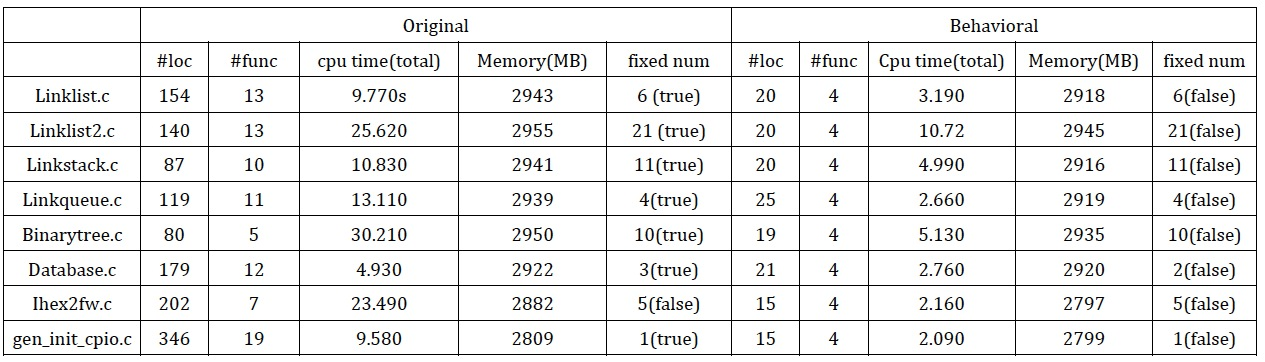
\includegraphics[width=14cm]{statistic.png}
%% \caption{Comparison}
%% \label{fig:statistic}
%% \end{figure}


\section{Related work}\label{sec:relatedwork}
Many methods for static memory-leak freedom verification have been
proposed~\cite{DBLP:conf/aplas/SuenagaK09,DBLP:conf/pldi/HeineL03,DBLP:conf/sigsoft/XieA05,DBLP:journals/scp/SwamyHMGJ06,DBLP:conf/sas/OrlovichR06,DBLP:conf/issta/SuiYX12}. These
methods guarantee partial memory-leak freedom and lack of illegal
accesses, whereas our type system guarantees total memory-leak
freedom. By using both their methods and our type system, we can
guarantee that a program correctly uses memory-allocation and
memory-deallocation primitives even if the program does not terminate.

Behavioral types are extensively studied in the context of concurrent
program
verification~\cite{DBLP:conf/esop/HondaVK98,DBLP:journals/tcs/IgarashiK04,DBLP:conf/esop/VieiraCS08,DBLP:journals/lmcs/KobayashiSW06}.
These type systems guarantee that the communication pattern of
concurrent programs are as intended.  Our type system is largely
inspired by one proposed by Kobayashi et
al.~\cite{DBLP:journals/lmcs/KobayashiSW06}, which guarantees that a
concurrent program accesses resources according to specification.

%% Model checking is a widely used technique for automatically verifying
%% correctness properties of finite-state
%% system~\cite{clarke1999model,ben2008principles,beyer2011cpachecker}. We
%% assume that some model checkers solves the constraints \(\OK_\nu(P)\)
%% in our paper. We expect that applying model checker to inferred
%% behavioral types is better than to the original programs, because a
%% behavioral type focuses on the actions related to allocations and
%% deallocations, abstracted away from other features. We plan to do some
%% experiments for this prospect.

One possible approach to total memory-leak freedom verification would
be checking that a program consumes only bounded number of memory
cells by using a model
checker~\cite{clarke1999model,ben2008principles,beyer2011cpachecker}.
We expect, from the result of the experiments, that the resource
required for model checking would become smaller if we apply a model
checker to the inferred behavior, which focuses on memory allocation
and deallocation.

\section{Conclusion}

We have described a type system to verify memory-leak freedom for
(possibly) nonterminating programs with manual memory-management
primitives where every memory cell is fixed size.  Our type system
abstracts the memory allocation/deallocation behavior of a program
with a CCS-like process with actions corresponding to memory
allocation and deallocation.  We have described a type reconstruction
algorithm for the type system.

Our current type system excludes many features of the real-world
programs for simplification.  We are currently investigating the C
programs in the real world to investigate what extension we need to
make to the type system.  One feature we have already noticed is
variable-sized memory blocks.  The current behavioral types ignores
the size of the allocated block, counting only the number of
\(\Malloc\) and \(\Free\), which makes the abstraction unsound for
actual programs.

Currently, our type reconstruction assumes that a model checker solves
constraints of the form \(\OK_n(P)\).  

%% type-based approach to safe memory deallocation
%% for non-terminating programs. The approach is based on the idea of
%% decomposing safe memory memory deallocation into partial correctness,
%% which is verified by previous type system, and behavioral
%% correctness. We designed a behavioral type system in our paper for
%% verification of behavioral correctness. Currently, we are looking for
%% a model checker to estimate an upper bound of consumption given a
%% behavioral type and planning to implement a verifier and conduct
%% experiment to see whether our approach is feasible.


\bibliographystyle{abbrv}
\bibliography{tan}

%\iffull
\newpage
\appendix
\section*{Appendix}

\section{Proof of Lemmas}
\label{sec:proof}

\begin{lemma}
\label{lem:okPreserved}
If \(\OK_n(P)\) and \(P \xlongrightarrow{\rho} P'\), then
\begin{itemize}
\item \(\OK_{n-1}(P')\) if \(\rho = \Malloc\),
\item \(\OK_{n+1}(P')\) if \(\rho = \Free\), and
\item \(\OK_n(P')\) if \(\rho = \tau\).
\end{itemize}
\end{lemma}
\begin{proof}

Case analysis on \(P \xlongrightarrow{\rho} P'\).

\begin{itemize}
\item Case $P = \TSKIP;P'$, \Rtab \(\TSKIP;P' \xlongrightarrow{\tau} P'\)

  We need to prove \(\OK_n(P')\).   We suppose that
  \(\OK_n(P')\) does not hold. Then, we have \(\TSKIP;P'
  \xlongrightarrow{\tau} P' \xlongrightarrow{\exists \rho}
  Q\), \(s.t.\) \(\sharp_{m}(\rho) - \sharp_{f}(\rho) > n\).

  From the definition of \(\OK_n(P)\), we have \(\sharp_m(\tau \cdot
  \rho) - \sharp_f(\tau \cdot \rho) \le n \). Then, we get
  \(\sharp_m(\tau) + \sharp_m(\rho) - \sharp_f(\tau) - \sharp_f(\rho)
  \le n\). From the definition of \(\sharp_\rho(\sigma)\), we have
  \(\sharp_m(\rho) - \sharp_f(\rho) \le n\). Therefore, we get the
  contradiction.

\item Case $P = \Malloc$, \Rtab \(\Malloc \xlongrightarrow{\Malloc} \TSKIP\)

%We need to prove \(\OK_{n-1}()
  
We need to prove \(\sharp_{m}(P') -
\sharp_{f}(P') \le n'\), where \(n'\) is \(n - 1\) and \(P'\) is \(\bf
0\). That is, we need to prove \( 1 \le n \).

 We have\(\ OK_{n}(\Malloc)\). From the definition of \(\OK_n(P)\),
 we have \(\sharp_{m}(\Malloc) - \sharp_{f}(\Malloc) \le
 n\). From the definition of \(\sharp_{\rho}(\sigma)\), we have
 \( 1 \le n\).

\item Case $P = \Free$

From the rule \rn{Sem-Free}, we need to prove \(\sharp_{m}(P') -
\sharp_{f}(P') \le n'\) where \(n'\) is \(n + 1\) and \(P'\) is \(\bf
0\). That is, we need to prove \( 0 \le n + 1\).

We have \(\OK_{n}(\Free)\). From the definition of \(\OK_n(P)\), we
have \(\sharp_{m}(\Free) - \sharp_{f}(\Free) \le n\). From the
definition of \(\sharp_{\rho}(\sigma)\), we have \( \ 0 \le n+1\).

\item Case $P = P_{1} + P_{2}$, \Rtab \(P_1 + P_2 \xlongrightarrow{\tau} P_1\)

  We prove \(\OK_n(P_1)\) by contradiction.  Assuming that
  \(OK_{n}(P_1)\) does not hold.  Then, we have \(P_{1} + P_{2}
  \xlongrightarrow{\tau} P_{1} \xlongrightarrow{\exists \rho} Q\),
  \(s.t.\) \(\sharp_{m}(\rho) - \sharp_{f}(\rho) > n\).

  From the definition of \(\OK_n(P)\),
  we have \(\sharp_m(\tau \cdot \rho) -\sharp_f(\tau \cdot \rho) \le
  n\). Then, we have \(\sharp_m(\tau) + \sharp_m(\rho) -
  \sharp_f(\tau) -\sharp_f(\rho) \le n\).  By the definition of
  \(\sharp_\rho(\sigma)\),  we get \(\sharp_m(\rho) -\sharp_f(\rho)
  \le n\). Therefore, we get the contradiction.

\item Case $P = P_{1} + P_{2}$, \Rtab \(P_1 + P_2 \xlongrightarrow{\tau} P_2\)

 The same to above.

\item Case $P = P_{1};P_{2}$

  We need to prove \(\OK_n(P_1)\).  To prove it by contradiction.
  Assuming that \(OK_{n'}(P_{1}';P_{2})\) does not hold. Then, we have
  \(P_{1};P_{2} \xlongrightarrow{\rho} P_{1}';P_{2}
  \xlongrightarrow{\exists \rho_1} Q\), \(s.t.\) \(\sharp_{m}(\rho_1)
  - \sharp_{f}(\rho_1) > n'\).

  From the definition of \(\OK_n(P)\), we have \( \sharp_{m}(\rho
  \cdot \rho_1) - \sharp_{f}(\rho \cdot \rho_1) \le n\).  We also have
  \(\sharp_{m}(\rho) + \sharp_{m}(\rho_1) - \sharp_{f}(\rho)
  -\sharp_{f}(\rho_1) \le n\).  From the assumption
  \(\sharp_{m}(\rho_1) - \sharp_{f}(\rho_1) > n'\), we have \infax{ n'
    + \sharp_m(\rho) - \sharp_f(\rho) < \sharp_{m}(\rho) +
    \sharp_{m}(\rho_1) - \sharp_{f}(\rho) -\sharp_{f}(\rho_1) \le n}

We have
$$
   n'=\left\{
   \begin{aligned}
     n + 1, && \rho = \Free \\
     n - 1,  && \rho = \Malloc  \\
     n ,      && otherwise
   \end{aligned}
   \right.
$$

   Hence, we have: if \(\rho = \Free\), then \(n + 1 - 1 < n\) from
   the definition of \(\sharp_{\rho}(\sigma)\); if \(\rho = \Malloc\),
   then \( n - 1 + 1 < n \); if \( \rho = other\), then \( n < n
   \). All of the three cases have \(n < n\). Therefore, we get the
   contradiction.

 \item Case  \(P = \mu\alpha.P'\),\Rtab  \( \mu\alpha.P' \xlongrightarrow{\tau} [\mu\alpha.P'\slash\alpha]P'\)

   We need to prove \(\OK_n([\mu\alpha.P'\slash\alpha]P')\).

   Considering the position of type variable \(\alpha\) in \(P'\), we need prove the following subcases:
$$
   P'=\left\{
   \begin{aligned}
     &P_1;\alpha,& \\
     &P_1;\alpha;P_2, and&  \\
     &\alpha;P_1&
   \end{aligned}
   \right.
$$

   \begin{itemize}
   \item Subcase \(P = \mu\alpha.P_1;\alpha\),\Rtab \(
     \mu\alpha.P_1;\alpha \xlongrightarrow{\tau} P_1;(\mu\alpha.P_1;\alpha) \)
     
     We need to prove \(\OK_n(P_1;(\mu\alpha.P_1;\alpha) \).

     By contradiction, we suppose that \( \mu\alpha.P_1;\alpha
     \xlongrightarrow{\tau} P_1;(\mu\alpha.P_1;\alpha)
     \xlongrightarrow{\exists \rho} Q s.t.  \sharp_m(\rho) -
     \sharp_f(\rho) > n\).

     We have \(\OK_n(P)\)).  By the definition of \(\OK_n(P)\), we
     have \(\sharp_m(\tau \cdot \rho) -\sharp_f(\tau \cdot \rho) \le
     n\). Hence, we have \(\sharp_m(\tau) + \sharp_m(\rho) -
     \sharp_f(\tau) -\sharp_f(\rho) \le n\).  From the definition of
     \(\sharp_\rho(\sigma)\), we have \(\sharp_m(\rho) -\sharp_f(\rho)
  \le n\). Therefore, we get the contradiction.

\item Subcase  \(P = \mu\alpha.P_1;\alpha;P_2\),\Rtab \(\mu\alpha.P_1;\alpha;P_2 \xlongrightarrow{\tau} P_1;(\mu\alpha.P_1;\alpha;P_2);P_2 \).

  We need to prove  \(\OK_n(P_1;(\mu\alpha.P_1;\alpha;P_2);P_2) \).

  By contradiction, the proof is similar to the above subcase.

     \item Subcase \(P = \mu\alpha.\alpha;P_1\),\Rtab
       \(\mu\alpha.\alpha;P_1 \xlongrightarrow{\tau}
       (\mu\alpha.\alpha;P_1);P_1 \).

       We need to prove \(\OK_n((\mu\alpha.\alpha;P_1);P_1)\).

       We can observe that this subcase is of the form like
       \(P\xlongrightarrow{\tau}P'\xlongrightarrow{\tau}P''\xlongrightarrow{\tau}
       \cdots\). Clearly, \(\OK_n(P')\) holds.

     \end{itemize}

\end{itemize}
\end{proof}

\begin{pfof}{Lemma~\ref{lem:preservation}}
By induction on the derivation of evaluation rules.\\

\begin{itemize}
\item Case: $\langle H, R, \FREE, n \rangle \xlongrightarrow{\Free}
  \langle H', R', \SKIP, n + 1 \rangle $.

We have \(\OK_n(P)\) and \(\Theta; \Gamma \vdash \Free(x) \COL P\).
From inversion of the typing rules, we have \(\Theta; \Gamma \vdash
\Free(x) \COL \Free\) and \(\Free \le P\) for some \(P'\).  Hence,
from the definition of subtyping, we have \(\TSKIP \le P''\) and \(P
\xLongrightarrow{\Free} P''\) for some \(P''\).

We need to find \(P_1\) such that \(P \xLongrightarrow{\Free} P_1\),
\(\Theta; \Gamma \vdash \SKIP \COL P_1\), and \(\OK_{n+1}(P_1)\).
Take \(P''\) as \(P_1\).  Then, \(P \xLongrightarrow{\Free} P''\) as
we stated above.  We also have \(\Theta; \Gamma \vdash \SKIP \COL
P''\) from \rn{T-Skip}, \(\TSKIP \le P''\), and \rn{T-Sub}.
\(\OK_{n+1}(P'')\) follows from Lemma~\ref{lem:okPreserved}.


\item Case: $\langle H, R, \LET x = \MALLOC \IN s, n \rangle
  \xlongrightarrow{\Malloc} \langle H', R', [x'/x]s, n - 1 \rangle
  $.

  From the assumption, we have \(\Theta; \Gamma \vdash \LET x =
  \MALLOC \IN s \COL P\) and \(\OK_{n}(P)\). By the inversion of
  typing rules, we have \(\Malloc;P_1 \le P\) and \(\Theta; \Gamma
  \vdash s : P_{1}\) for some \(P_1\). We have the following
  derivation: \infrule{ \Malloc \xlongrightarrow{\Malloc} 0}
  {\Malloc;P_1 \xlongrightarrow{\Malloc} 0;P_{1}} and \(0;P_1
  \rightarrow P_{1}\), then we have \(\Malloc;P_{1}
  \xLongrightarrow{\Malloc} P_{1}\). Hence, By the definition of
  subtyping, we have \(P \xLongrightarrow{\Malloc}P''\) and \(P_{1}
  \le P''\) for some \(P''\)

  We need to find \(P'\) such that \(\Theta; \Gamma' \vdash
  [x'/x]s\COL P'\),\(P\xLongrightarrow{\Malloc} P'\). Take \(P''\) as
  \(P'\). Then \(P \xLongrightarrow{\Malloc} P''\) as we state above. We
  also have \(\Theta;\Gamma \vdash [x'/x]s \COL P''\) from \rn{T-Sub},
  \(\Theta;\Gamma \vdash [x'/x]s \COL P_1\) and \(P_1 \le
  P''\). \(\OK_{n-1}(P'')\) follows from Lemma~\ref{lem:okPreserved}.

\item Case: $\langle H, R, \SKIP;s, n \rangle \rightarrow \langle
  H, R, s, n \rangle $.

  we have \(\Theta;\Gamma \vdash \SKIP;s\COL  P\) and
  \(\OK_{n}(P)\). From the inversion of the typing rules, we have
  \(\Theta; \Gamma \vdash s\COL P_{1}\) and \(0;P_{1} \le
  P\). Hence, from the definition of subtyping, we have \(P
  \xLongrightarrow{\tau} P''\) and \(P_{1} \le P''\) for some \(P''\).

  We need to find \(P'\) such that \(\Theta; \Gamma \vdash s : P'\)
  and \(P \xLongrightarrow{\tau} P'\). Take \(P''\) as \(P'\). Then \(P
  \xLongrightarrow{\tau} P''\) as we stated above. We also have
  \(\Theta;\Gamma \vdash s\COL P''\) from \rn{T-Sub}, \(\Gamma \vdash
  s\COL P_{1}\) and \(P_{1} \le P''\). \(\OK_n(P'')\) follows from
  Lemma~\ref{lem:okPreserved}

\item Case: $\langle H, R, *x \leftarrow y , n \rangle \rightarrow
  \langle H', R', \SKIP, n \rangle $.

  We have \(\Theta; \Gamma \vdash *x \leftarrow y : P\) and
  \(\OK_{n}(P)\). From the inversion of typing rules, we have \(0 \le
  P\).

  We need to find $P'$ such that \(\Theta; \Gamma \vdash \SKIP: P'\),
  \(P \xLongrightarrow{\tau} P'\) and \(\OK_n(P')\). Take $P$ as $P'$. Then,
  \(P \xLongrightarrow{\tau} P'\) and \(\OK_n(P')\) hold. We also have \(\Theta;
  \Gamma \vdash \SKIP: P'\) from \rn{T-Skip}, \(0 \le P\) and
  \rn{T-Sub}.

\item Case: $\langle H, R, \LET x = y\ \IN s , n \rangle
  \rightarrow \langle H', R', [x'/x]s, n \rangle $.

  We have \(\Theta; \Gamma \vdash \LET x = y\ \IN \ s \COL P\) and
  \(OK_{n}(P)\). From the inversion of typing rules, we have \(\Theta;
  \Gamma \vdash s\COL P_{1}\) and \(P_{1} \le P\).

  We need to find $P'$ such that \(\Theta; \Gamma \vdash [x'/x]s : P'\) ,
  \(P \xLongrightarrow{\tau} P'\) and \(\OK_n(P'\)). Take \(P\) as
  \(P'\). Then \( P \xLongrightarrow{\tau} P'\) and \(\OK_n(P')\) hold.  We
  also have \(\Theta; \Gamma \vdash [x'/x]s\COL P\) from \rn{T-Sub},
  \(\Theta; \Gamma \vdash [x'/x]s\COL P_{1}\) and \( P_{1} \le
  P\).

\item Case: $\langle H, R, \LET x = \NULL \ \IN \ s, n \rangle
  \rightarrow \langle H', R', [x'/x]s, n \rangle $

  We have \(\Theta; \Gamma \vdash \LET x = \NULL \ \IN \ s\COL P\)
  and \(OK_{n}(P)\). From the inversion of typing rules, we have
  \(\Theta; \Gamma \vdash s\COL P_{1}\) and \( P_{1} \le P\).

  We need to find $P'$ such that \(\Theta; \Gamma' \vdash [x'/x]s\COL P'\),
  \(P \xLongrightarrow{\tau} P'\) and \(\OK_n(P')\).  Take \(P\) as
  \(P'\).  Then, \(P \xLongrightarrow{\tau} P'\) and \(\OK_n(P')\) hold.  We
  also have \(\Theta; \Gamma \vdash [x'/x]s\COL P\) from \rn{T-Sub},
  \(\Theta; \Gamma \vdash [x'/x]s\COL P_{1}\)\( P_{1} \le
  P\). 

\item Case: $\langle H, R, \LET x = *y \ \IN \ s, n \rangle
  \rightarrow \langle H', R', [x'/x]s, n \rangle $

  We have \(\Theta; \Gamma \vdash \LET x = *y \ \IN \ s\COL  P\) and
  \(OK_{n}(P)\). From the inversion of typing rules, we have \(\Theta;
  \Gamma \vdash s\COL P_{1}\) and \(P_{1} \le P\).

  We need to find \(P'\) such that \(\Theta; \Gamma \vdash [x'/x]s\COL
  P'\), \(P \xLongrightarrow{\tau} P'\) and \(\OK_n(P')\). Take \(P\) as
  \(P'\). Then, \(P \xLongrightarrow{\tau} P'\) and \(\OK_n(P')\) hold.  We
  also have \(\Theta; \Gamma' \vdash [x'/x]s\COL P\) from \rn{T-Sub},
  \(\Theta; \Gamma' \vdash [x'/x]s\COL P_{1}\) and \(P_{1} \le P\).
        
\item Case(\rn{Tr-IfNullT}): \(\langle H, R, \IFNULL \Cirx \ \THEN s_{1} \ \ELSE \ s_{2},
  n \rangle \rightarrow \langle H, R, s_{1}, n \rangle\)

  We have \(\Theta; \Gamma \vdash \IFNULL \Cirx \ \THEN \ s_{1}
  \ \ELSE \ s_{2}\COL P\) and \(\OK_{n}(P)\). From the inversion of
  typing rules, we have \(\Theta; \Gamma \vdash s_{1} : P_{1}\) and \(P_{1}
  \le P\).

  We need to find $P'$ such that \(\Theta; \Gamma \vdash s_1\COL P'\)
  , \(P \xLongrightarrow{\tau} P'\) and \(\OK_n(P'\)).  Take P as P'.  Then,
  \(\OK_n(P')\) and \(P \xLongrightarrow{\tau} P'\) hold. We also have \(\Theta;
  \Gamma' \vdash s_{1}\COL P\) from \(\Theta; \Gamma \vdash s_{1}\COL
  P_1\), \(P_{1} \le P\) and \rn{T-Sub}.

\item Case(\rn{Tr-IfNullF}): \(\langle H, R, \IFNULL \Cirx \ \THEN s_{1} \ \ELSE \ s_{2},
  n \rangle \rightarrow \langle H, R, s_{2}, n \rangle\).

 The proof is similar to case \rn{Tr-IfNullT}. 

\item Case: $\langle H, R, f(\vec{x}) , n \rangle \rightarrow  \langle H, R, [\vec{x}/\vec{y}]s, n  \rangle $

  Assuming that \(D(f) = s\) and \(\Theta(f) = P_1\), we have \(s\COL
  P_1\). The \([\vec{x}/\vec{y}]s\) also has a type \(P_1\).

  From the assumption, we have \(\Theta;\Gamma \vdash f(x)\COL P\) and
  \(\OK_n(P)\). From the inversion, we have \(\Theta;\Gamma \vdash
  f(x)\COL P_1\) and \(P_1 \le P\).

  We need to find \(P'\) such that \(\Theta;\Gamma \vdash [\vec{x}/\vec{y}]s\COL
  P'\), \(P \xLongrightarrow{\tau} P'\) and \(\OK_n(P')\). Take \(P\) as
  \(P'\). Then \(P \xLongrightarrow{\tau} P'\) and \(\OK_n(P')\) hold. We
  also have \(\Theta;\Gamma \vdash [\vec{x}/\vec{y}]s\COL P \) from
  \(\Theta;\Gamma \vdash [\vec{x}/\vec{y}]s\COL P_1\), \(P_1 \le P\) and
  \rn{T-Sub}.

\end{itemize}

\end{pfof}

\section{Syntax Directed Typing Rules}

Typing rules showed in Figure are not immediately suitable for type
inference. The reason is that the subtyping rule can be applied to any
kind of term. This means that, any kind of term $s$ can be applied by
either subtyping rule or the other rule whose conclusion matches the
shape of the $s$ \cite{plain:book1}.

In order to yield a type inference algorithm, we should do something with the subtyping rule. The method is to merge the subtyping rule with the other rules by introducing a set $C$ of constraints, where $C$ consists of subtype constraints on behavioral types of the form $P_{1}\le P_{2}$ and $OK_{n}(P)$.

Syntax directed typing rules are listed in Figure 

$$
     \frac{ C = \emptyset}
           {\Theta; \Gamma; C \vdash \SKIP : \mathbf{0}}
      \Rtab \mbox{(ST-Skip)}
$$
$$
      \frac{\Theta;\Gamma ; C_{1} \vdash s_{1} : P_{1} \Rtab \Theta; \Gamma ; C_{2} \vdash s_{2} : P_{2} \Rtab C = C_{1}\cup C_{2} \cup \{ P_{1};P_{2} \le P\}}
      {\Theta;\Gamma; C \vdash s_{1};s_{2} : P}
      \Rtab \mbox{(ST-Seq)}
$$
$$
      \frac{\Theta;\Gamma;C_{1} \vdash y \Rtab \Theta;\Gamma; C_{2} \vdash x : \mathbf{Ref} \Rtab C = C_{1}\cup C_{2}}
      {\Theta;\Gamma; C \vdash *x \leftarrow y : \mathbf{0}}
      \Rtab \mbox{(ST-Assign)}
$$
$$
      \frac{C = \emptyset}
      {\Gamma ; C \vdash \Free() : \Free}
     \Rtab \mbox{(ST-Free)}
$$
$$
     \frac{\Theta;\Gamma, x ; C_{1} \vdash s : P_{1} \Rtab C = C_{1} \cup\{P_{1}\le P\}}
     {\Theta;\Gamma; C \vdash \LET x = \Malloc() \; \IN s : \Malloc ; P}
     \Rtab \mbox{(ST-Malloc)}
$$
$$
     \frac{\Theta;\Gamma; C_{1} \vdash y \Rtab \Theta;\Gamma, x ; C_{2} \vdash s : P_{1} \Rtab C = C_{1}\cup C_{2} \cup \{P_{1} \le P \}}
     {\Theta;\Gamma ; C \vdash \LET x = y \;  \IN s : P}
     \Rtab \mbox{(ST-LetEq)}
$$
$$
     \frac{\Theta;\Gamma ; C_{1} \vdash y: \mathbf{Ref} \Rtab \Theta;\Gamma, x ; C_{2} \vdash s : P_{1} \Rtab C = C_{1}\cup C_{2}\cup\{P_{1} \le P\}}
     {\Theta;\Gamma ; C \vdash \LET x = *y \; \IN s : P}
     \Rtab \mbox{(ST-LetDref)}
$$
$$
     \frac{\Theta;\Gamma; C_{1} \vdash x \Rtab \Theta;\Gamma; C_{2} \vdash s_{1} : P_{1} \Rtab \Theta;\Gamma; C_{3} \vdash s_{2} : P_{2}  \Rtab  C = C_{1} \cup C_{2} \cup C_{3} \{P_{1}\le P, P_{2}\le P \}}
     {\Theta;\Gamma; C \vdash \IFNULL\Cirx \THEN s_{1} \ELSE s_{2} : P }
    \; \;  \mbox{(ST-IfNull)}
$$
$$
     \frac{\Theta(f) = P_{1} \Rtab C = P_{1} \le P}
     {\Gamma,\vec{x}:\vec{\tau} \vdash f(\vec{x}) : P }
     \Rtab \mbox{(ST-Call)}
$$
$$
     \frac{\Theta \vdash D : \Theta \Rtab \Theta ; \emptyset ; C_{1} \vdash s : P \Rtab C = C_{1}\cup\{OK_{n}(P)\}}
     {C \vdash (D , s) }
     \Rtab \mbox{(ST-Program)}
$$
$$
    \mathbf{Figure \; 5.} \;\; \mbox{Syntax Directed Typing Rules}
$$

\section{Typing Inference Algorithm}

\begin{figure}
\begin{nospaceflalign*}
   PT_{\Theta}(f) &  =  &\\
  & \ \  \LET  \alpha = \Theta(f) & \\
  & \ \ \IN   (C = \{\alpha \le \beta \}, \beta) &
\end{nospaceflalign*}
\begin{nospaceflalign*}
   PT_{\Theta}(\SKIP) &  =  (\emptyset, 0)&
\end{nospaceflalign*}
\begin{nospaceflalign*}
   PT_{\Theta}(s_{1}&;s_{2})  =  &\\
   & \ \ \ \LET (C_{1}, P_{1}) = PT_{\Theta}(s_{1}) & \\
   &\ \ \ \ \ \ \  \ (C_{2}, P_{2}) = PT_{\Theta}(s_{2}) & \\
   & \ \ \ \IN   (C_{1} \cup C_{2}\cup \{P_{1}; P_{2} \le \beta \}, \beta) &
\end{nospaceflalign*}
\begin{nospaceflalign*}
   PT_{\Theta}(*x& \leftarrow y)   =  &\\
  & \ \ \LET (C_{1}, \emptyset) = PT_{v}(*x) & \\
  & \ \ \ \ \ \ (C_{2}, \emptyset) = PT_{v}(y) & \\
  &\ \  \IN    (C_{1} \cup C_{2},  0) &
\end{nospaceflalign*}
\begin{nospaceflalign*}
   PT_{\Theta}(\Free(x)) &  = (\emptyset, \Free)  &
\end{nospaceflalign*}
\begin{nospaceflalign*}
   PT_{\Theta}(\LET &x = \Malloc() \  \IN s)  =  &\\
   &\LET (C_{1}, P_{1}) = PT_{v}(s) & \\
   &\IN  (C_{1} \cup \{P_{1} \le \beta \} ,  \Malloc; \beta) &
\end{nospaceflalign*}
\begin{nospaceflalign*}
   PT_{\Theta}(\LET &x = y \  \IN s )  =  &\\
   &  \LET (C_{1}, \emptyset) = PT_{v}(y) & \\
   & \ \ \ \ \ (C_{2}, P_{1}) = PT_{\Theta}(s) & \\
   &  \IN   (C_{1} \cup C_{2}\cup \{P_{1} \le \beta \},  \beta) &
\end{nospaceflalign*}
\begin{nospaceflalign*}
   PT_{\Theta}(\LET &x = *y \  \IN s )  =  &\\
   & \LET  (C_{1}, \emptyset) = PT_{v}(y) & \\
   &\ \ \ \ \ \ (C_{2}, P_{1}) = PT_{\Theta}(s) & \\
   & \IN   (C_{1} \cup C_{2}\cup \{P_{1} \le \beta \},  \beta) &
\end{nospaceflalign*}
\begin{nospaceflalign*}
   PT_{\Theta}(&\IFNULL(x) \  \THEN  s_{1} \  \ELSE \ s_{2} )  =  &\\
   & \ \ \ \ \ \LET  (C_{1}, P_{1}) = PT_{\Theta}(s_{1}) & \\
   &\ \ \ \ \  \ \ \ \ \ (C_{2}, P_{2}) = PT_{\Theta}(s_{2}) & \\
   &\ \ \ \ \  \ \ \ \ \ (C_{3}, \emptyset) = PT_{v}(x) & \\
   & \ \ \ \ \ \ \IN   (C_{1} \cup C_{2}\cup C_{3}\cup \{P_{1} \le \beta, P_{2} \le \beta \},  \beta) &
\end{nospaceflalign*}
\begin{nospaceflalign*}
   PT(\langle D, s \rangle&)   =  &\\
   &\LET  \Theta = \{ f_{1}:\alpha_{1}, \dots, f_{n}:\alpha_{n}  \} &\\
   & \ \ \ \ \  where \ \{ f_{1},\dots, f_{n} \} = dom(D) \ and \ \alpha_{1}, \dots, \alpha_{n} \  are \ fresh  & \\
   & \IN    \LET  (C_{i}, P_{i}) = PT_{\Theta}(D(f_{i})) \  for \  each \ i & \\
   & \IN    \LET  C_{i}^{'} = \{ \alpha_{i} \le P_{i} \} \ for \  each \ i & \\
   & \IN    \LET  (C, P) = PT_{\Theta}(s)  & \\
   & \IN   (C_{i} \cup C_{i}^{'} ) \cup C \cup  \{OK(P)\},  P) &
\end{nospaceflalign*}
\caption{Type Inference Algorithm}
\label{fig:tyin}
\end{figure}

%\else
%\fi

\end{document}
